\chapter{基于多维度特征的子痫前期识别模型的构建与分析}
\section{引言}
本章在第四章构建中的PPG多维度时域特征集(PPGMTFS)与PPG采样值时域特征集(PPGSTFS)的基础上,按照基于波形(PR)与基于被试(SR)等两个研究方向,
利用ML的多种监督学习算法,完成了PE识别模型的构建与分析工作。本章首先介绍了两种典型的ML监督学习算法原理与常用作评估模型优劣的性能指标。随后,在进行具体的PE识别模型的构建时,
完成了包括多算法模型筛选、模型超参数优化、特征贡献度分析与降维处理等研究分析工作。最后,基对上述分析过程得到的具体模型的性能的数值进行了对比,并分析总结了基于PPG进行PE识别模型的
研究过程中得到的基本结论。本章研究内容的框架图如\autoref{fig:frameworks5}所示。

\begin{figure}[htbp]
      \centering
      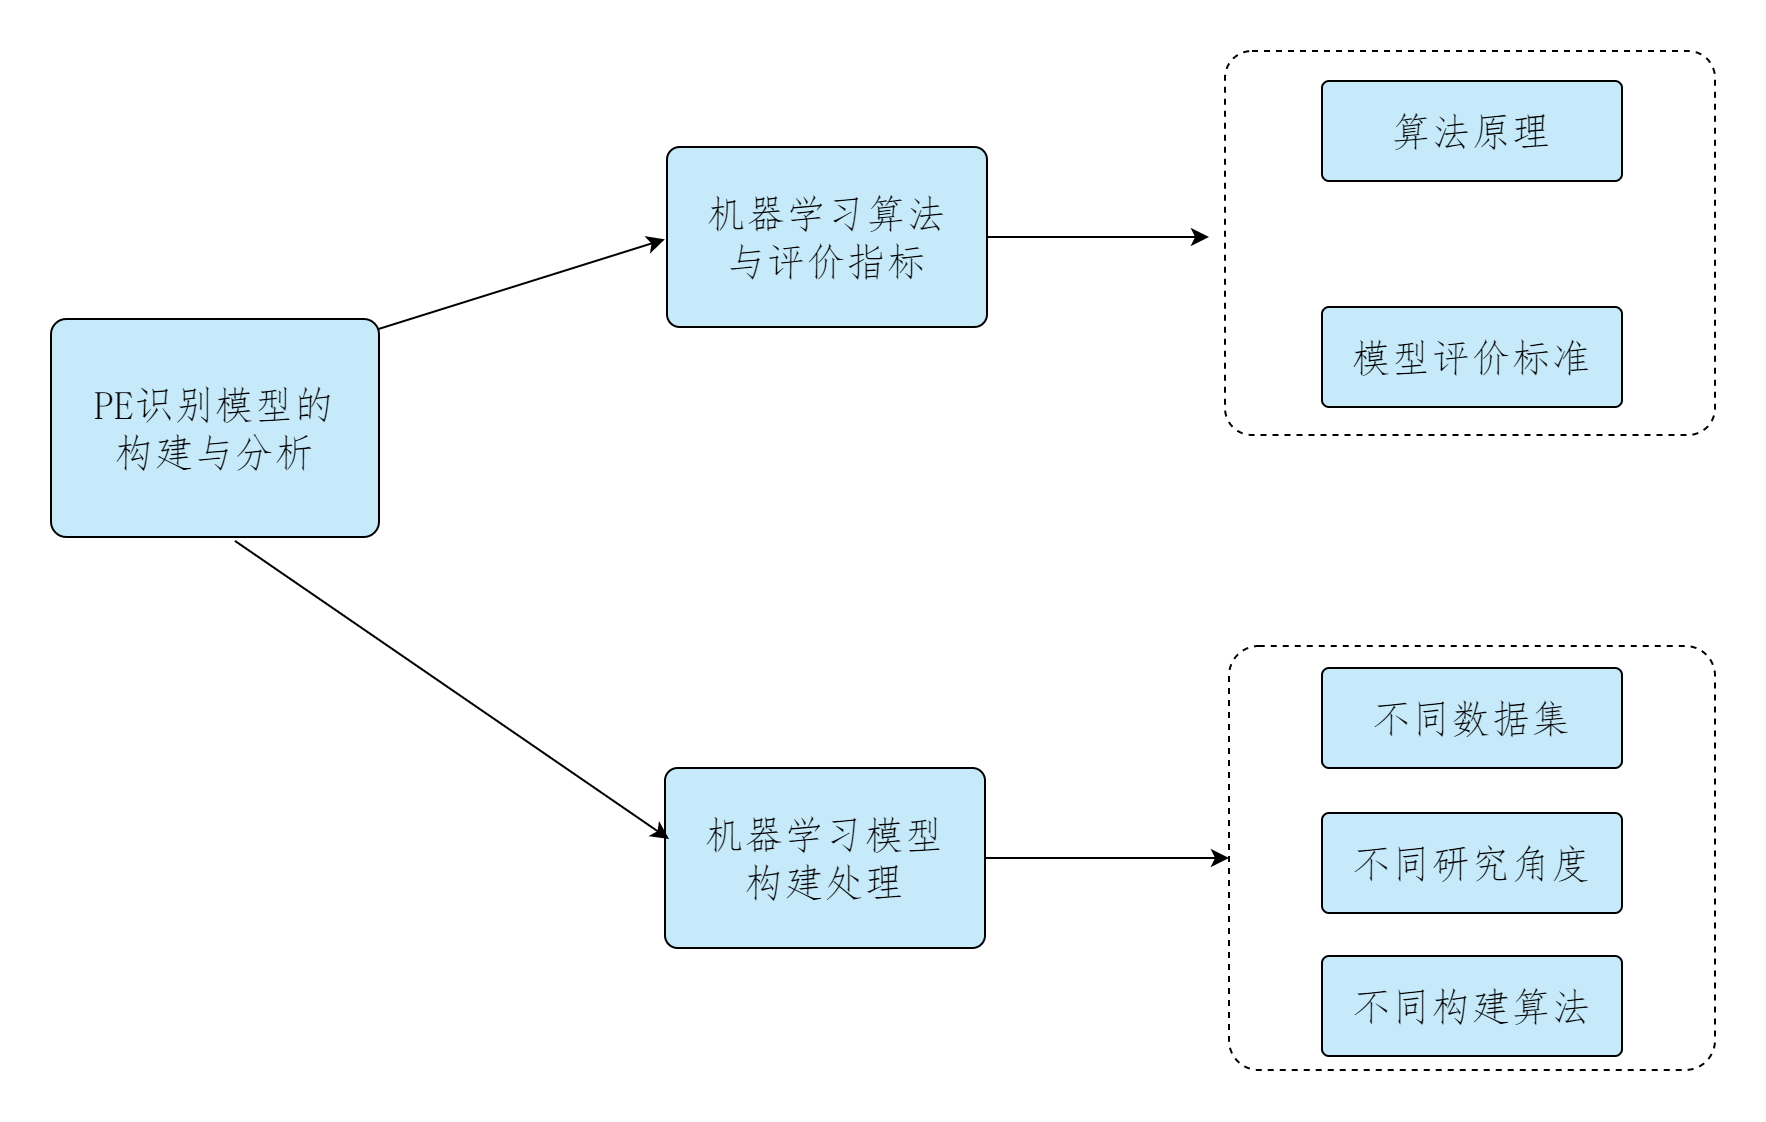
\includegraphics[width=\linewidth]{results/frameworks5}
      \caption{\label{fig:frameworks5}第五章研究内容框架}
\end{figure}
\vspace{-0.8cm} 

\section{机器学习算法原理与模型评价标准}
一般认为,ML是一门致力于研究通过计算的手段、利用已有的经验来改善系统自身性能的学科和艺术\cite{Zhou2016,Aurélien2018}。Tom Mitchell对ML给出了一种最为经典的形式化定义:
计算机程序利用经验$E$学习任务$T$,其性能是$P$,如果针对任务$T$的性能$P$随着经验$E$不断增长,此时可以断言,关于$T$与$P$,该程序对$E$进行了学习\cite{mitchell1997,Zhou2016}。
对计算机程序而言,$E$通常以数据的形式存在,因此,ML可以视为从数据中产生模型的算法过程,不显式编程是ML的最典型特征。

尽管Tom Mitchell关于ML的概念在上世纪五十年代就已经被提出,但直到进入新世纪后,ML才真正迎来井喷式发展的黄金期。
由于半导体电子计算机行业的充分发展,人们收集、传输、处理数据的能力均取得了长足的进步,各种社会活动中出现的海量数据也因此具备了能够被挖掘、分析的硬件基础与需要被分析并加以利用的客观需求。
在此背景下,ML受到了学者们的广泛关注并进入了蓬勃发展阶段,不论是抽象的数学理论基础,还是具体情景下的应用研究,ML均取得了重大突破。
目前,ML技术在模式识别、数据挖掘、自然语言处理、语言识别、图像识别、芯片设计、信息检索及生物信息学等学科领域得到广泛应用,
尤其为交叉学科的发展提供了新的技术支撑与突破点\cite{Zhou2016,Aurélien2018,Li2017}。   

本小节介绍了两种有代表性的ML算法原理,同时也对几种常用于评价ML模型的性能指标进行了说明。

\subsection{决策树与随机森林的算法原理}
监督学习是ML的重要研究方向,主要用于推断观察数据与目标变量之间的潜在关系。其中,观察输入也被称为输入数据,而目标变量也被称为因变量或数据标签。
基于监督学习算法,良好训练的函数模型可以准确预测出隐藏在不熟悉与未观察到的数据实例中的类标签。

本研究的后续使用的所有ML算法均属监督学习范畴,下面以决策树(decision tree,DT)算法与随机森林(random forest,RF)算法为代表进行原理介绍。

一、DT

DT是数据挖掘的经典算法之一,可用于连续数值型变量的回归预测及离散型数值型变量的分类问题\cite{Li2017,Liu2018}。
DT是一种类似流程图的树结构,其最显著优点是简单直观,易于可视化、可读性强。

1、DT的结构与原理

DT是对实例进行分类的树形结构的描述,由结点和有向边组成,而结点又可分为内部结点与叶节点,如\autoref{fig:dt}所示。其中,结点表示一个特征或属性;有向边则对应着决策结果,一般是一个数据标签类\cite{Li2017,Zhou2016}。
DT可以看成一个if-else规则的集合,DT的根节点到叶节点的每条路径分别对应着一条规则:路径上的内部结点集合构成了规则的判断条件,而叶节点所属的具体类则对应着该规则的结论。
D的学习目的就是从训练数据集中集中归纳出一组分类规则,产生一颗与训练数据的矛盾小的、泛化能力强的逻辑判断树。
\begin{figure}[htbp]
      \centering
      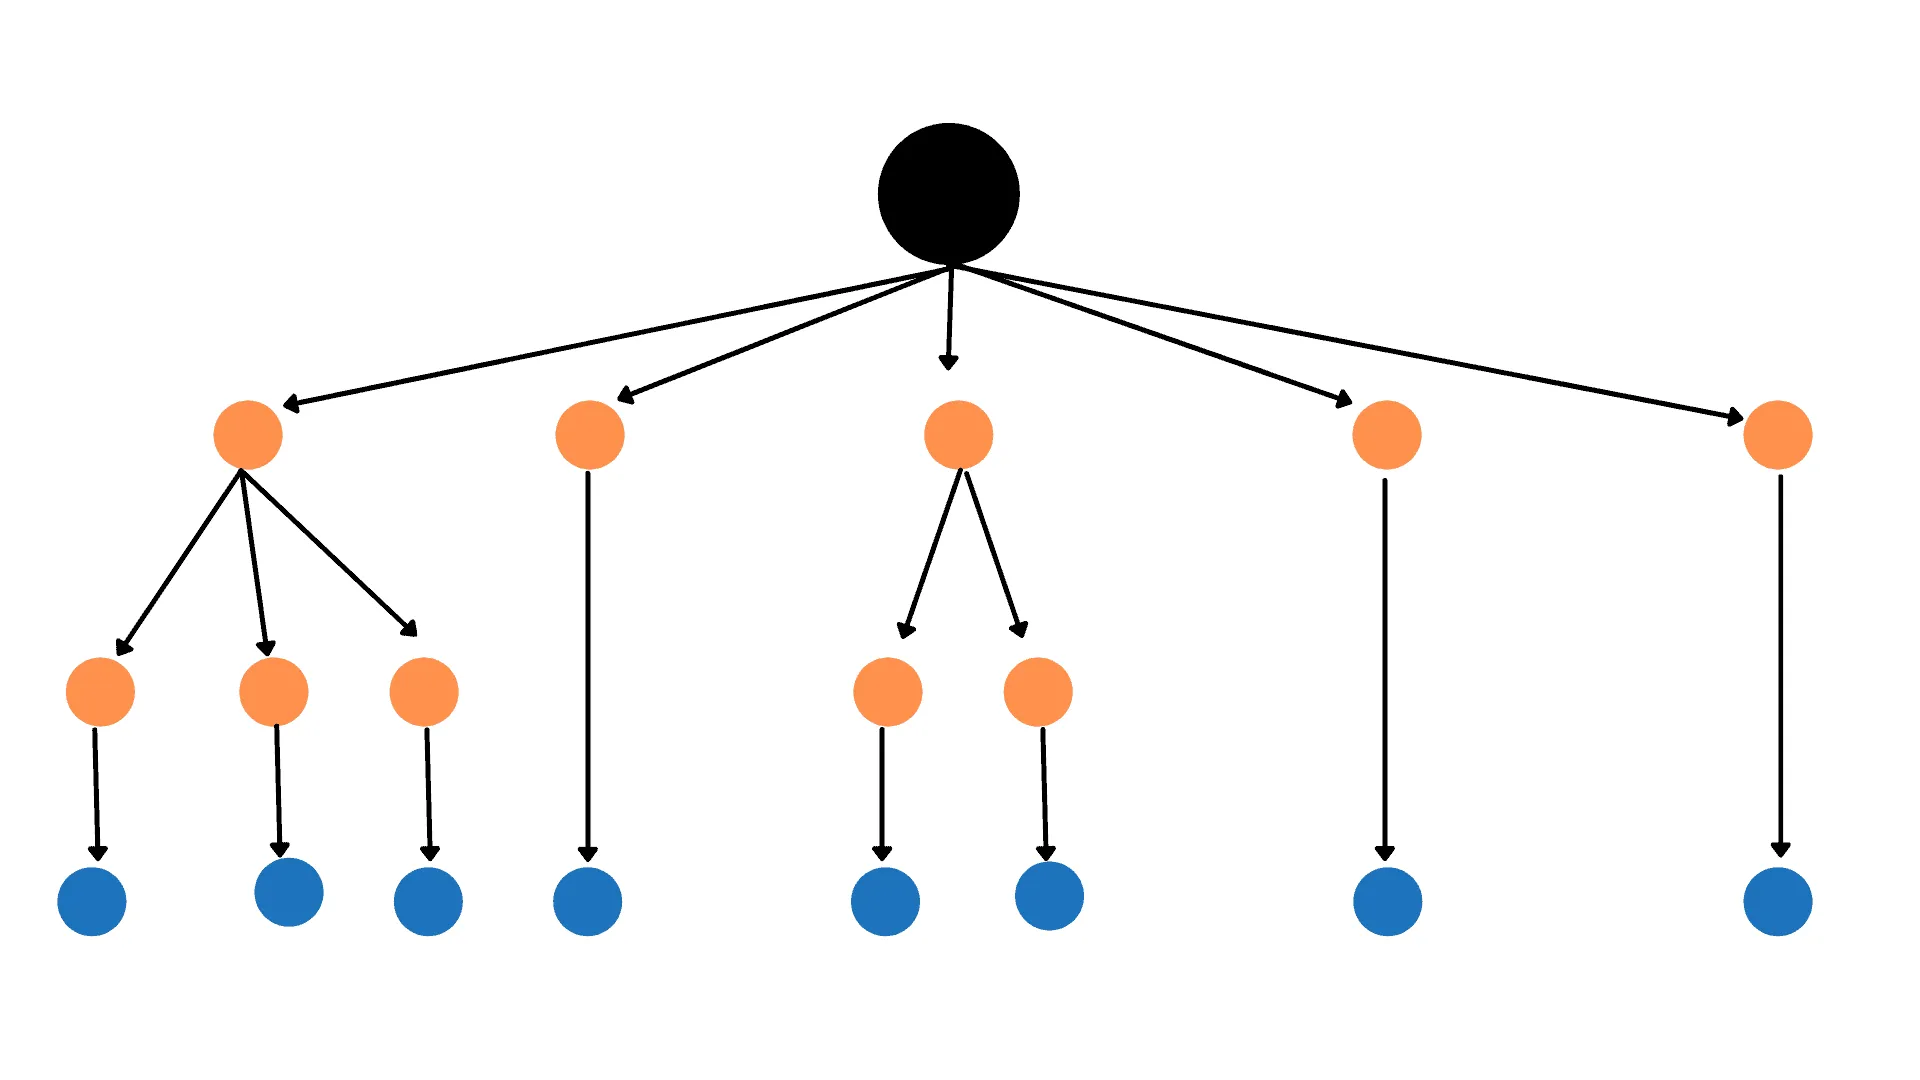
\includegraphics[width=.6\linewidth]{models/dt.png}
      \caption{\label{fig:dt}决策树模型示意}
\end{figure}

2、DT的特征选择

为生成一颗分类能力强的DT,一种可行的策略是只选取对分类效果有提升的特征参与构建。基尼指数(Gini index,GI)与信息增益(information gain,IG)是两种最常用的用于筛选最佳特征的指标。

GI也称为基尼不纯度,其定义为
\begin{equation}
      \label{equ:gini}
      G_i = 1 - \sum_{k=1}^n{p_{i,k}}^2
\end{equation}
其中,$p_{i,k}$是第$i$个节点上,类别为$k$的训练实例占比。GI数值越大,样本集合的不确定性也越大。特别地,对于样本集合$D$,根据特征$A$是否取某一具体可能值$a$,将$D$分割成$D_1$和$D_2$两部分,即
\begin{equation}
      \label{equ:daset}
      \left \{
      \begin{aligned}
            D_1 &= \{ (x,y) \in D \mid A(x) = a\} \\
            D_2 &= D - D_1
      \end{aligned}
      \right.
      \end{equation}
那么,在特征$A$的条件下,样本集合的GI可以表示为
\begin{equation}
      \label{equ:ginia}
      G(D,A) = \frac{|D_1|}{|D|}G(D_1) + \frac{|D_2|}{|D|}G(D_2)
\end{equation}
其中,$|D|$表示样本集合$D$的样本数量。\autoref{equ:ginia}描述了$D$经特征$A=a$分割后的不确定性。此时,筛选最佳特征可以转换为寻找使\autoref{equ:ginia}取值最小的特征$A$的具体数值。

IG是在信息论中的信息熵(information entropy,IE)概念基础上进行定义使用的,其具体含义与使用方法与上文介绍的GI类似,这里不再进行赘述\cite{Zhou2016,Li2017}。

3、DT的生成

DT的生成构建过程就是递归地选择最优特征,并根据最优特征对训练数据进行分割,使该分割对各个新的子数据集有最优分类效果的过程。其中,DT的经典生成算法包括第三代迭代二分器(iterative dichotomiser 3,ID3)算法、
第4.5代分类器(classifier 4.5,C4.5)算法及分类与回归树(classification and regression tree,CART)算法等\cite{quinlan1986,quinlan1993,breiman1984}。
其中,只有CART算法可以同时应用于分类任务与回归任务的DT生成过程,故CART算法的应用也最为广泛。

CART算法采用最小GI来选择特征,生成的决策树为二叉树,其工作的基本原理如\autoref{alg:cart}所示。
\begin{breakablealgorithm}
      \caption[CART生成算法]{CART递归生成算法\cite{Li2017}}
      \label{alg:cart}
      \begin{algorithmic}[1] %每行显示行号
            \Require 训练数据集$D$。
            \Ensure 分类回归树CART。
            \State 建立一颗空树$CART$,设该树的根结点为$root$。
            \Function{GenerateCart}{$CART,D_c,root$}
                  \State $D_c$为当前结点的训练数据集,计算现有特征对该数据集的GI。对每一个特征$A$,对其可能取的每个值$a$,根据样本点对$A=a$的测试为“是”或“否”将$D_c$分割成$D_l$与$D_r$两部分,使用\autoref{equ:ginia}计算$A=a$时的GI。
                  \State 在所有可能的特征$A$以及它们所有可能的切分点$a$中,选择GI最小的特征及其对应的切分点作为最有特征与最优切分点。
                  \State 依最优特征与最优切分点,从现结点生成两个子节点$left$与$right$,将训练数据集依特征分配到两个子节点中去,即$D_l$与$D_r$。更新当前$CART$。
                  \If {结点中的样本个数小于预定阈值 \textbf{or} 样本集的GI小于预定阈值 \textbf{or} 没有更多特征}
                  \State \Return{$CART$}
                  \Else    
                  \State \Call{GenerateCart}{$CART,D_l,left$}
                  \State \Call{GenerateCart}{$CART,D_r,right$}
                  \EndIf
            \EndFunction
      \end{algorithmic}
\end{breakablealgorithm}

4、DT的剪枝

为防止DT出现生长过于茂密后对训练数据过拟合,通常都会对DT的生长进行剪枝(pruning)处理。DT的剪枝方法可以分为预剪枝与后剪枝两大类。
前者的工作原理是在DT的生长阶段就对其进行一定的限制,包括限制树最大生长深度、限制DT生成的最多叶节点数量等。
后剪枝则是在DT得到完全生长之后进行,其处理算法也更复杂、训练时间等开销也更大\cite{Zhou2016,Liu2018}。

二、RF

RF是一种在套袋法(bagging)基础上发展起来的集成学习算法,最早由Leo Breiman于2001年提出\cite{breiman2001}。

1、Bagging

为获得泛化性能强的不同的基学习器,一种可行的策略是对所有学习器使用同一种训练算法,但是在训练集的不同随机子集上进行训练,使这些基学习器的能够有一定的差异,\autoref{fig:bp}所示。
在上述过程的随机子集的建立过程中,若对原始数据样本的采样后放回,这种方法即为bagging;与之对应的,采样后不放回的方法称为粘贴法(pasting)\cite{Aurélien2018,Zhou2016}。
由于bagging法可以获得的随机子集数量远远高于pasting法,其应用范围也更加广泛。
\begin{figure}[htbp]
      \centering
      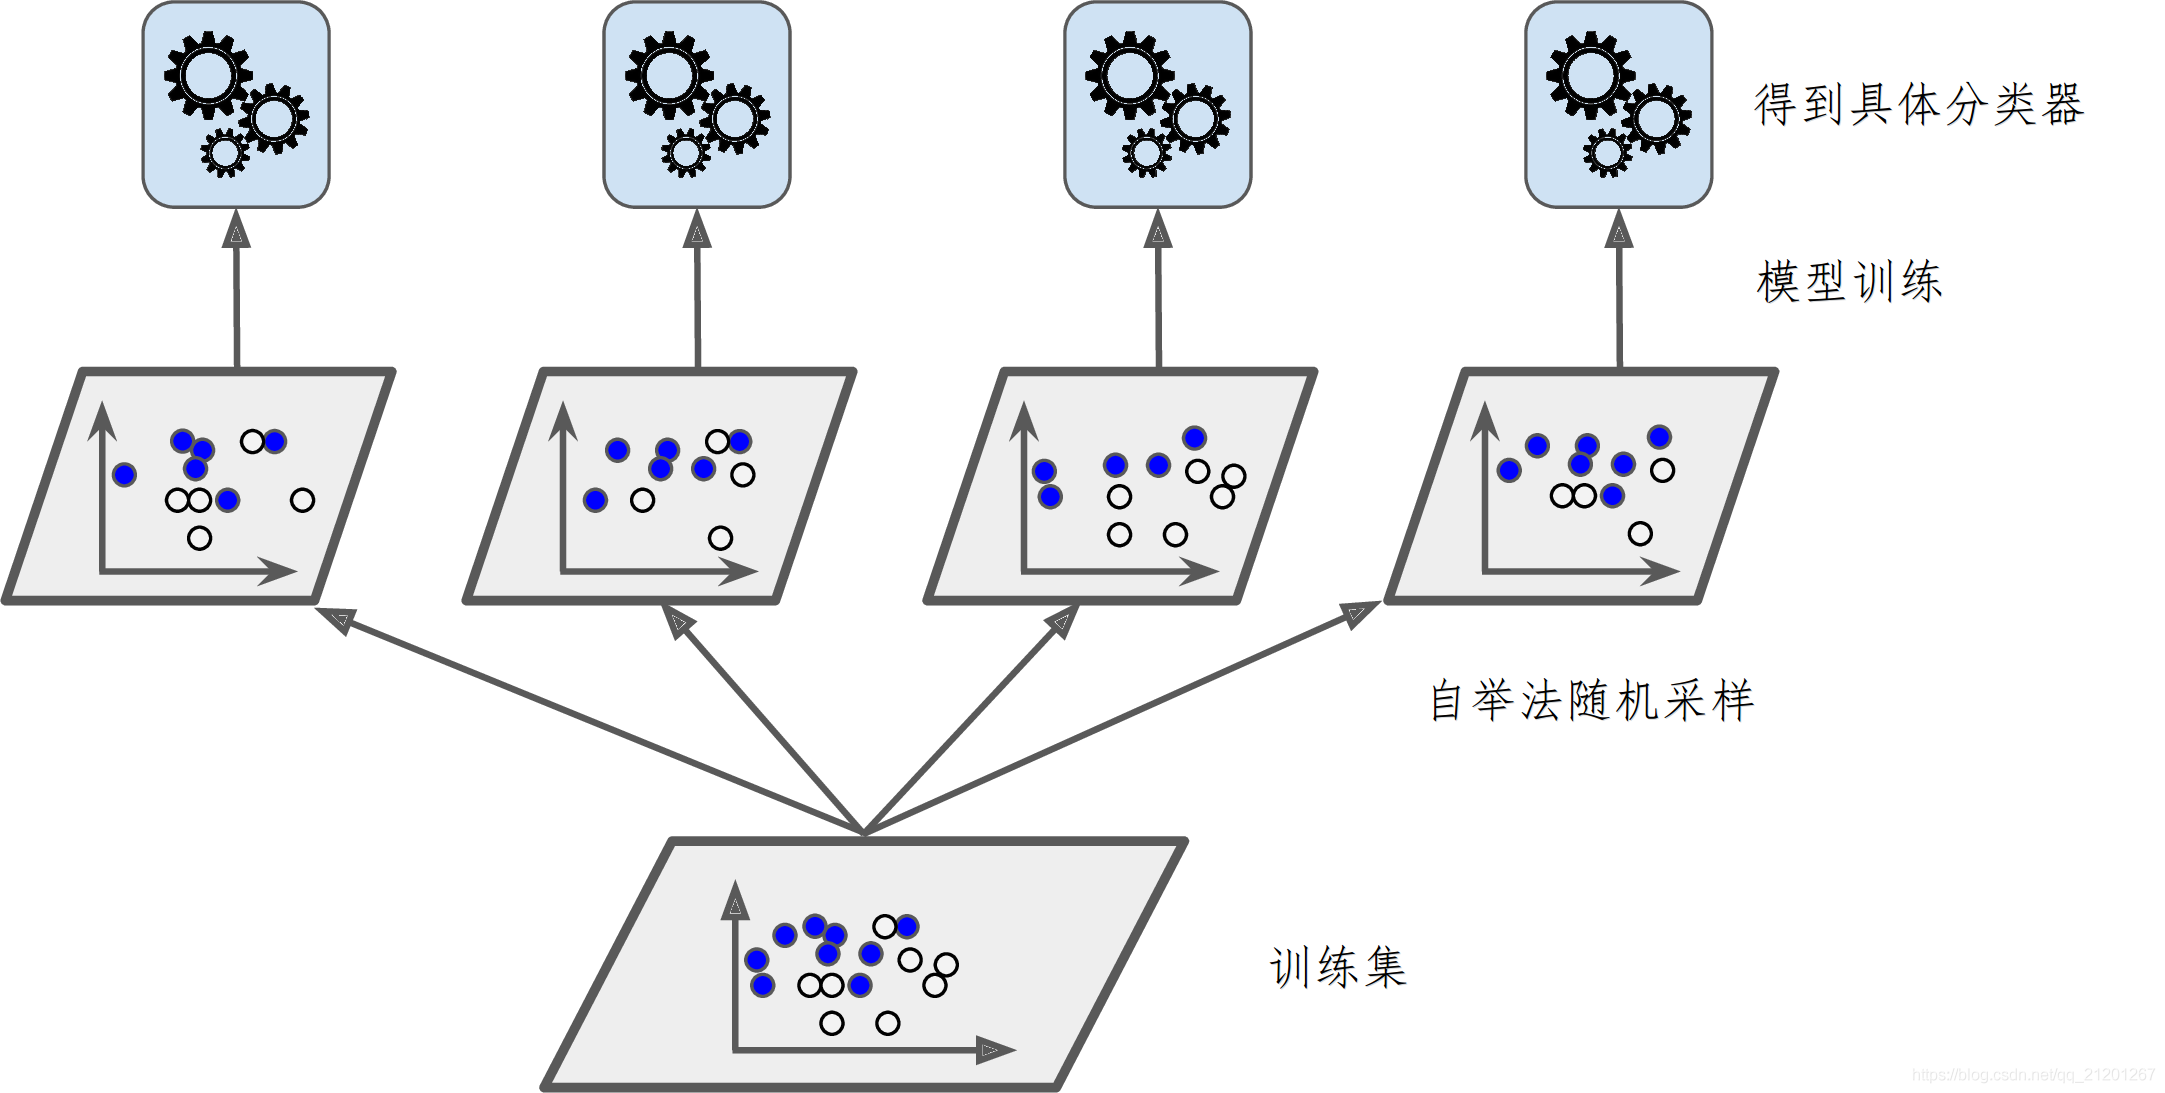
\includegraphics[width=.8\linewidth]{models/bp}
      \caption[Bagging与pasting示意]{\label{fig:bp}Bagging与pasting示意\cite{Aurélien2018}}
\end{figure}

当使用有采样后即放回的方法从包含$m$个原始样本的训练集$D$抽取出$m$个新的样本构成此次训练数据集$D_{bs}$时,显然,$D$有部分数据样本在$D_{bs}$重复出现,部分数据则从未被抽样过。
由概率与统计知识可知,特定样本在$m$次抽取后,从未被抽中的概率为$(1-\frac{1}{m})^m$。当$m \to \infty$时,可得
\begin{equation}
      \label{equ:me}
      \lim_{m \to \infty}{(1-\frac{1}{m})}^m = \frac{1}{e} \approx 0.368
\end{equation}
这说明约有36.8\%的原始样本未出现在采样集$D_{bs}$中,这部分数据可以作为当前训练算法的测试集。

按上述思想,可从原始样本训练集$D$采样得到$T$个包含$m$个训练样本的采样集,基于这些采样集,使用特定的机器学习算法可以训练得到$T$个基学习器,结合这些基学习器的输出即为bagging算法
的基本流程,如\autoref{alg:bagging}所示。投票法和平均法是bagging在进行基学习器的输出时常采用的策略。
\begin{breakablealgorithm}
      \caption[Bagging算法]{Bagging算法\cite{Zhou2016}}
      \label{alg:bagging}
      \begin{algorithmic}[1] %每行显示行号
            \Require 训练集$D=\{(x_1,y_1),(x_2,y_2),\dots,(x_m,y_m)\}$;基学习算法$\xi$;训练轮数$T$。
            \Ensure $H(x)=\arg \max \limits_{y \in Y} \sum_{t=1}^T \mathbb{I}(h_t(x)=y)$,其中$\mathbb{I}(.)$为指示函数,在$.$为真或假时函数值分别为1或0。
            \For {$t=1,2,\dots,T$}
                  \State 从原始训练集$D$自助采样得到此次的样本分布$D_{bs}$
                  \State $h_t=\xi (D,D_{bs})$
            \EndFor
      \end{algorithmic}
\end{breakablealgorithm}

2、RF

RF是由多棵DT构成,这些DT一般都是经过充分生长的、未经剪枝处理的CART,如\autoref{fig:rf}所示。
而“随机”一词有两重含义,首先是同Bagging算法一样,每棵DT在训练时使用的训练样本是随机抽取的;其次,与\autoref{alg:cart}所示的一般CART生成算法不同,RF中的CART
在生长时并不是在当前结点的$d$个属性集合$A$中选取最优特征及其最优切分点,而是先从$A$中随机生成一个包含$k$个属性子集的$A_{bs}$,随后再从$A_{bs}$中选择最优属性进行划分\cite{Zhou2016,Liu2018,breiman2001}。其中,$k$的推荐取值为
$\lfloor \log_2m + 1 \rfloor$\cite{breiman2001}。

\begin{figure}[htbp]
      \centering
      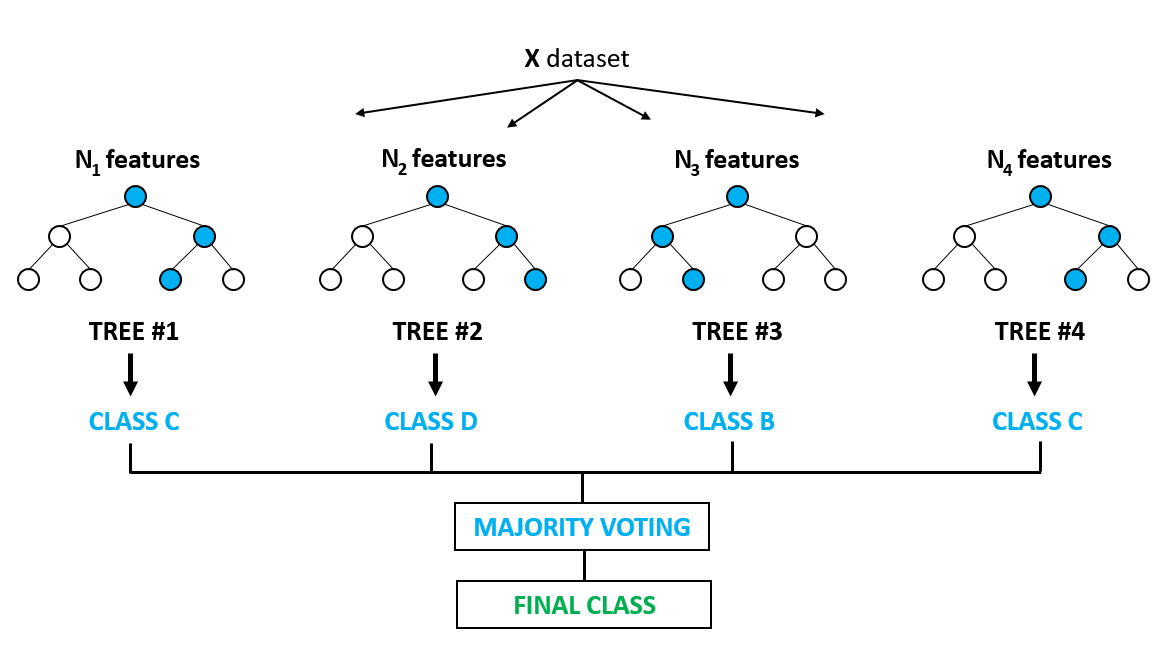
\includegraphics[width=.8\linewidth]{models/rf}
      \caption{\label{fig:rf}RF示意}
\end{figure}

对回归问题而言,RF的输出是其中所有DT的输出的均值;而对分类任务而言,RF的输出是所有DT输出的投票结果。RF在树的生长过程中的两次随机使DT具有更大的多样性,相当于用更高的偏差换取更低的方差。因此,
最终的集成结果有着出色的泛化性能,有效避免了使用单棵DT可能导致的过拟合问题。RF算法运行速度快、准确率高且泛化性能优秀,被誉为“代表集成学习技术水平的方法”\cite{Zhou2016,Liu2018}。

另外,RF也被应用于特征筛选的相关问题中\cite{Aurélien2018}。重新考察\autoref{fig:dt}中的DT可以发现,越靠近根结点位置的特征对决策过程的重要程度也越高,而不重要的特征多出现在靠近结点的位置、甚至不出现在DT中。
因此,特征的重要性(或贡献度)可以通过其在RF众多DT中的平均深度来进行量化衡量。

\subsection{机器学习模型的评价标准}
本小节对常用于量化ML算法模型的性能指标进行了介绍。

一、混淆矩阵及其衍生指标

混淆矩阵(confusion matrix,CM)是评估分类器分类效果优劣的常用工具\cite{Zhou2016,Aurélien2018}。其总体思路就是分别统计A类别实例被划分成B类别实例的数目。理论上CM的行列数目没有上限,而在实际应用中,
二分类任务的CM是最常见的。

对二分类任务对应的CM而言,人们习惯将样例依据其真实所属类别与分类器预测类别的四种组合结果进行命名,即真阳性(true positive,TP)、假阳性(false positive,FP)、真阴性(true negative,TN)
及假阴性(false negative,TN),如\autoref{tab:cm}所示。显然,$TP+FP+TN+FN=\text{样例总数}$。
\begin{center}
      \zihao{-5}
      \begin{longtable}{m{3cm}<{\centering}m{3cm}<{\centering}m{3cm}<{\centering}}
      \caption{二分类任务的混淆矩阵}\\
      \label{tab:cm}\\
      \topline
      \colorhead  & \multicolumn{2}{c}{\textbf{预测结果}} \\
      \colorhead \multirow{-2}{*}{\textbf{真实情况}}  & 阳性(1) & 阴性(0)\\
      \midline
      \endfirsthead
      \caption[]{(续)}\\
      \topline
      \colorhead  & \multicolumn{2}{c}{\textbf{预测结果}} \\
      \colorhead \multirow{-2}{*}{\textbf{真实情况}}  & 阳性(1) & 阴性(0)\\
      \midline
      \endhead 
      \hline
      \endfoot
      \bottomline
      \endlastfoot
      \colorrowa 阳性(1) & 真阳性(TP) & 假阴性(FN) \\
      \colorrowc 阴性(0) & 假阳性(FP) & 真阴性(TN) \\
\end{longtable}
\end{center}

\vspace{-0.8cm}
由于CM是按类型进行统计的绝对数值,为量化分类器的具体性能,人们在CM的基础上衍生定义了一系列数字指标,包括查全率(recall)、查准率(precison)、准确率(accuracy)及特异性(specificity)等,
如\autoref{equ:measures}所示。
\begin{equation}
      \label{equ:measures}
      \left \{
      \begin{aligned}
            \text{Recall}      &=\frac{\text{TP}}{\text{TP+FN}}         \\
            \text{Precison}    &=\frac{\text{TP}}{\text{TP+FP}}          \\
            \text{Accuracy}    &=\frac{\text{TP+TN}}{\text{TP+FP+TN+FN}} \\
            \text{Specificity} &=\frac{\text{TN}}{\text{TN+FP}}       \\
      \end{aligned}
      \right.
\end{equation}

查全率亦称召回率、灵敏性(sensitivity)或真阳性率(true positive rate,TPR),查准率亦称精准率,特异性亦称真阴性率。查全率与查准率是应用的最广泛的两个指标\cite{Zhou2016,Aurélien2018}。
而查全率与查准率是对相互矛盾的度量指标,一个指标性能的提高意味着另一个指标性能的下降,这称为精度-召回率权衡。通常只有在简单分类任务中,
才能同时获得较高的查准率与查全率。

为评估查全率与查准率均不相等的分类器性能,人们进一步定义了$F_1$值
\begin{equation}
      \label{equ:f1}
      \begin{aligned}
            F_1   &= \frac{2}{\frac{1}{\text{Precison}}+\frac{1}{\text{Recall}}}         \\
                  &=\frac{2\cdot \text{Precison}\cdot \text{Recall}}{\text{Precison+Recall}}          \\
                  % &=\frac{TP}{TP+\frac{FN+FP}{2}} \\
      \end{aligned}
\end{equation}
$F_1$值是召回率与精准率的谐波均值,召回率与精准率相近的分类器易获得更高的$F_1$值。

在评估分类器性能时需要根据场景,从\autoref{equ:measures}与\autoref{equ:f1}中灵活选取恰当的评价指标。

二、ROC曲线、AUC与约登指数

ROC曲线是另一种常用于二分类问题的分析工具。ROC绘制的是真阳性率和假阳性率(false positive rate,FPR)之间的变化关系,其中
\begin{equation}
      \label{equ:fpr}
      \text{FPR}=\frac{\text{TN}}{\text{TN+FP}}=1-\text{Specificity}
\end{equation}
因此,ROC曲线也被称为灵敏度与1$-$特异性曲线。绘制曲线时,以分类器的预测结果对样例进行升序排列,依次将样本作为阳性进行预测。计算对应的TPR与FPR后,可得一坐标点$(\text{FPR},\text{TPR})$,最后将所有坐标点连线即可,如\autoref{fig:roc}所示。
其中,虚线表示纯随机分类器的ROC曲线,理想性能的分类器应无限逼近左上角,即坐标点$(0,1)$。
\begin{figure}[htbp]
      \centering
      \includegraphics[width=.6\linewidth]{data_plan/roc}
      \caption[ROC曲线与AUC关系]{\label{fig:roc}ROC曲线与AUC关系}
\end{figure}

在衡量多个分类器性能优劣时,常将分类器对应的ROC曲线下面积AUC作为判据。纯随机分类器ROC曲线对应的AUC数值为0.5,而理想分类器ROC曲线的AUC数值为1,如\autoref{fig:roc}所示。

此外,约登指数(Youden index,YI)也是用来评价分类器效果的一个指标。若在评估分类器性能时,给予将分类器假阴性和假阳性以相同权重,即可应用约登指数
\begin{equation}
      \label{equ:yi}
      \begin{aligned}
            \text{YI}&=\text{Sensitivity}-(1-\text{Specificity})\\
            &=\text{Sensitivity}+\text{Specificity}-1
      \end{aligned}
\end{equation}
一般认为,当YI取值最大时,此时对应的分类阈值为最佳阈值\cite{cwl}。

\section{基于PPG多维度时域特征集的机器学习分析}
本小节基于第四章提出的PG多维度时域特征集(PPGMTFS),围绕基于PPG波形(PR)与基于被试(SR)等两个研究方向,利用多种ML算法,进行了PE识别分析模型的相关研究。
\subsection{基于PPG波形的研究}
PR将单个PPG波形作为分析识别PE的最小分析对象,认为PPG的波形是孕妇PE病发状态的稳定“表达”,单个PPG波形包含了可以识别区分PE的全部信息。
PR使用了第四章提及的对波形分层抽样的数据作为训练集与测试集。在此基础上,进行了ML算法初筛、算法超参数优化及特征贡献度分析与特征降维等研究工作。

一、算法初筛

本研究使用了九种监督学习的算法进行了PE识别模型的前期研究,具体包括随机梯度下降(stochastic gradient descent,SGD)、决策树(decision tree,DT)、K近邻(K-nearest neighbors,KNN)、
高斯朴素贝叶斯(Gaussian plain Bayes,GPB)、逻辑回归(logistic regression,LR)、线性支持向量机(linear support vector machines,LSVM)、核支持向量机(kernel support vector machines,KSVM)、
C-支持向量机(C-support vector machines,CSVM)及多层感知机(multilayer perceptron,MLP)等九种分类算法。

前期研究未对上述算法的超参数进行调整,全部使用默认数值或推荐数值\cite{scikit-learn}。
通过这些算法训练得到的ML模型(以下简称为模型)在训练集与测试集上的结果如\autoref{tab:model_screen}所示,其中训练集的统计结果是经5层交叉验证处理后得到的,而一些需要注意的数据信息也在\autoref{tab:model_screen}
用粉色底色进行了突出显示。
\begin{center}
      \zihao{-5}
      \begin{longtable}{m{1.5cm}<{\centering}m{1cm}<{\centering}m{1cm}<{\centering}m{1cm}<{\centering}m{1cm}<{\centering}m{1cm}<{\centering}m{1cm}<{\centering}m{1cm}<{\centering}m{1cm}<{\centering}m{1cm}<{\centering}m{1cm}<{\centering}}
            \caption{初筛结果}\\
            \label{tab:model_screen}\\
            \topline
            \colorhead &  & \multicolumn{5}{c}{\textbf{训练集}} & \multicolumn{4}{c}{\textbf{验证集}}                                                                                                                                                                                                      \\
            \colorhead \multirow{-2}{*}{\textbf{模型类型}} & \multirow{-2}{*}{\textbf{训练时间}} &  \textbf{精确率} &  \textbf{召回率} &  \textbf{F1值} &  \textbf{准确率} &  \textbf{AUC}  &  \textbf{精确率} &  \textbf{召回率} &  \textbf{F1值} &  \textbf{准确率}    \\
            \midline
            \endfirsthead
            \caption[]{(续)}\\
            \midline
            \colorhead &  & \multicolumn{5}{c}{\textbf{训练集}} & \multicolumn{4}{c}{\textbf{验证集}}                                                                                                                                                                                                      \\
            \colorhead \multirow{-2}{*}{\textbf{模型类型}} & \multirow{-2}{*}{\textbf{训练时间}} &  \textbf{精确率} &  \textbf{召回率} &  \textbf{F1值} &  \textbf{准确率} &  \textbf{AUC}  &  \textbf{精确率} &  \textbf{召回率} &  \textbf{F1值} &  \textbf{准确率}    \\
            \midline
            \endhead 
            \midline
            \endfoot
            \bottomline
            \endlastfoot
            \colorrowa SGD      &   6.17 s   & 87.2\% & 68.9\% & 77.0\% & 75.5\% & 0.876 & \cellcolor{pink} 74.8\% & 97.7\% & 84.7\% & 79.0\% \\
            \colorrowc DT       &   5.24 s  & 91.1\% & 83.0\% & 86.9\% & 85.1\% & 0.907 & 93.6\% & 81.4\% & 87.1\% & 85.6\% \\
            \colorrowa KNN      &   3.08 s    & \cellcolor{pink} 94.7\% & \cellcolor{pink} 93.7\% & \cellcolor{pink} 94.2\% & \cellcolor{pink} 93.1\% & \cellcolor{pink} 0.974  & 95.4\% & 93.3\% & 94.3\% & 93.3\% \\
            \colorrowc GNB      &   \cellcolor{pink}1.22 s  & 87.9\% & 63.9\% & 74.0\% & 73.2\% & \cellcolor{pink}0.838  & 90.1\% & \cellcolor{pink} 65.0\% & 75.5\% & 74.9\% \\
            \colorrowa LR       &   \cellcolor{pink}203.0 s  & 90.2\% & 90.7\% & 90.4\% & 88.6\% & 0.950 & 93.3\% & 93.0\% & 93.1\% & 91.8\% \\
            \colorrowc LSVM     &   47.22 s  & 79.7\% & 93.2\% & 86.0\% & 81.9\% & 0.917 & 95.9\% & 81.9\% & 88.3\% & 87.1\% \\
            \colorrowa KSVM     &   60.28 s  & 82.5\% & 90.3\% & 86.2\% & 82.8\% & 0.916 & 84.9\% & 91.4\% & 88.0\% & 85.2\% \\
            \colorrowc CSVM     &   42.47 s  & 84.3\% & 90.5\% & 87.3\% & 84.3\% & 0.929 & 87.1\% & 90.8\% & 88.9\% & 86.5\% \\
            \colorrowa MLP      &   26.8 s  & 83.5\% & 75.8\% & 79.5\% & 76.6\% & 0.905 & 89.3\% & 91.1\% & 90.2\% & 88.2\% \\
      \end{longtable}
\end{center}

从\autoref{tab:model_screen}中的具体数值可以得到以下结论:

1、从模型的训练时间方面来看,GNB算法训练所需时间最短,仅需1.22s,而MLP、LSVM、KSVM与CSVM算法所需时间较长,LR算法训练时间最长为203.0s。这些数值也与各算法的
复杂度对应,符合预期。

2、从模型在测试集上AUC方面来看,只有GNB算法得到的模型AUC数值在0.850以下,而由KNN算法得到的AUC最高可达为0.974。

3、从各模型在训练集上的精度-召回率权衡上来看,由KNN与LR算法得到的模型表现最好,精确率、召回率及F1数值均在90.0\%以上。由DT、LSVM、KSVM与CSVM等算法得到的模型在精确率与召回率可以达到90.0\%+80.0\%
(或80.0\%+90.0\%)以上,这些模型的F1值也均在86.0\%以上。而由SGD、GNB与MLP算法得到的模型在这些数值上表现较差。

4、从各模型在验证集上的泛化能力来看,由SGD与GNB算法得到的模型性能最差,出现精确率或召回率数值小于75\%的情况,而由另外七种算法得到的模型泛化能力较强。其中,由DT、LR、LSVM、KSVM、CSVM与MLP算法得到的模型性能接近,精确率与召回率可以达到90.0\%+80.0\%
(或80.0\%+90.0\%),F1值也均在87.0\%以上。而由KNN与LR算法得到的模型表现最为优秀,精确率、召回率与F1值三者数值更是均在93.0\%以上。

5、上述数值结果初步说明了PPGMTDS包含了一定数量的与PE相关性较强的特征参数。
而对初筛阶段探索使用的九种机器学习算法而言,通过KNN与LR算法构建的PE识别模型的性能最为出色,而由SGD与GNB算法得到的模型性能最差。

二、初筛模型的超参数优化

超参数(Hyperparameter)是指ML模型在开始学习过程之前人工设置值的调优参数\cite{scikit-learn,Aurélien2018},而超参数的调整与优化通常会使模型的性能得到一定的提升。
网格搜索是寻找最优超参数最为常用的策略之一,其基本原理为预先设置好该算法的所有待调超参数的可选值集合,通过排列组合的方式得到该算法的多个实例后,
使用这些算法实例分别在训练集上训练模型,在测试集上的性能最优的模型使用的超参数组合即为全局最优超参数\cite{Aurélien2018}。
而判断性能最优可使用多种参数指标,各模型在训练集上的AUC数值是其中最为常见的一种。

由于上步模型初筛时,\autoref{tab:model_screen}中的数值结果是在各算法使用默认超参数的条件下得到的,因此,本研究也对这些算法的最优超参数进行了研究。
在综合考虑模型的训练时间及初筛性能表现等因素,本研究选取了初筛阶段有代表性的SGD、GNB、DT与KNN等四种算法进行了超参数优化。
其中,由前两类算法训练得到的模型在初筛阶段性能较差,超参数优化是为了探索显著提升其性能的可能;由后两类算法训练得到的模型在初筛阶段表现较好,超参数优化是为了探索其最佳性能。

\autoref{tab:super_para}给出了上述四种算法给出了在进行网格搜索时各超参数的值域组合与最优超参数数值。其中,超参数组合值域一栏加粗显示了各模型的超参数的默认数值,而最优超参数是以各模型在测试集上的AUC取值为衡量标准得到的。
与此同时,\autoref{fig:contrast_model}也对比展示了在超参数优化前后,各模型在训练集上的AUC数值及在测试集上准确率变化情况,其中,AUC数值是在测试集上进行5层交叉验证后求均值得到的。

\begin{center}
      \zihao{-5}
      \begin{longtable}{m{4cm}<{\centering}m{6.5cm}<{\centering}m{4cm}<{\centering}}
            \caption{初筛模型的超参数优化}\\
            \label{tab:super_para}\\
            \topline
            \colorhead \textbf{模型类型} & \textbf{超参数组合值域}     &     \textbf{最优超参数}\\
            \midline
            \endfirsthead
            \caption[]{(续)}\\ 
            \midline
            \colorhead \textbf{模型类型} & \textbf{超参数组合值域}     &     \textbf{最优超参数}\\
            \endhead 
            \midline
            \endfoot
            \bottomline
            \endlastfoot
            \colorrowa SGD    & \begin{tabular}[c]{@{}l@{}}loss:{[}\textbf{hinge}, log\_loss,   \\ log, modified\_huber, \\ squared\_hinge, perceptron, \\ squared\_error,  huber,\\  epsilon\_insensitive, \\ squared\_epsilon\_insensitive{]},\\    penalty:{[}\textbf{l2},l1,elasticnet{]},\\   alpha:{[}0.001,\textbf{0.0001},0.00001{]}\end{tabular} &  \begin{tabular}[c]{@{}l@{}}alpha=0.001, \\ loss=squared\_hinge,   \\ penalty=elasticnet\end{tabular}     \\
            \colorrowc GNB   & var\_smoothing:{[}1e-5,1e-7,\textbf{1e-9},1e-11{]}             & var\_smoothing=1e-7                     \\
            \colorrowa DT          & \begin{tabular}[c]{@{}l@{}}criterion:{[}\textbf{gini},entropy,log\_loss{]},\\  splitter:{[}\textbf{best},random{]},\\     max\_depth:{[}\textbf{3},4,5{]},\\  max\_features:{[}sqrt,log2,\textbf{None}{]}\end{tabular}        & \begin{tabular}[c]{@{}l@{}}criterion=entropy,\\ splitter=random,\\ max\_depth=5, \\ max\_features=None\end{tabular}         \\
            \colorrowc KNN           & \begin{tabular}[c]{@{}l@{}}n\_neighbors:{[}3,\textbf{5},7,9{]},\\    weights:{[}\textbf{uniform},distance{]}\end{tabular}       & \begin{tabular}[c]{@{}l@{}}n\_neighbors=9,\\  weights=distance\end{tabular}             \\
      \end{longtable}
\end{center}
\vspace{-0.8cm}

\begin{figure}[htbp]
      \centering
      \subfigure[\label{fig:cmdl1}各模型在超参数优化前后的性能对比]{
      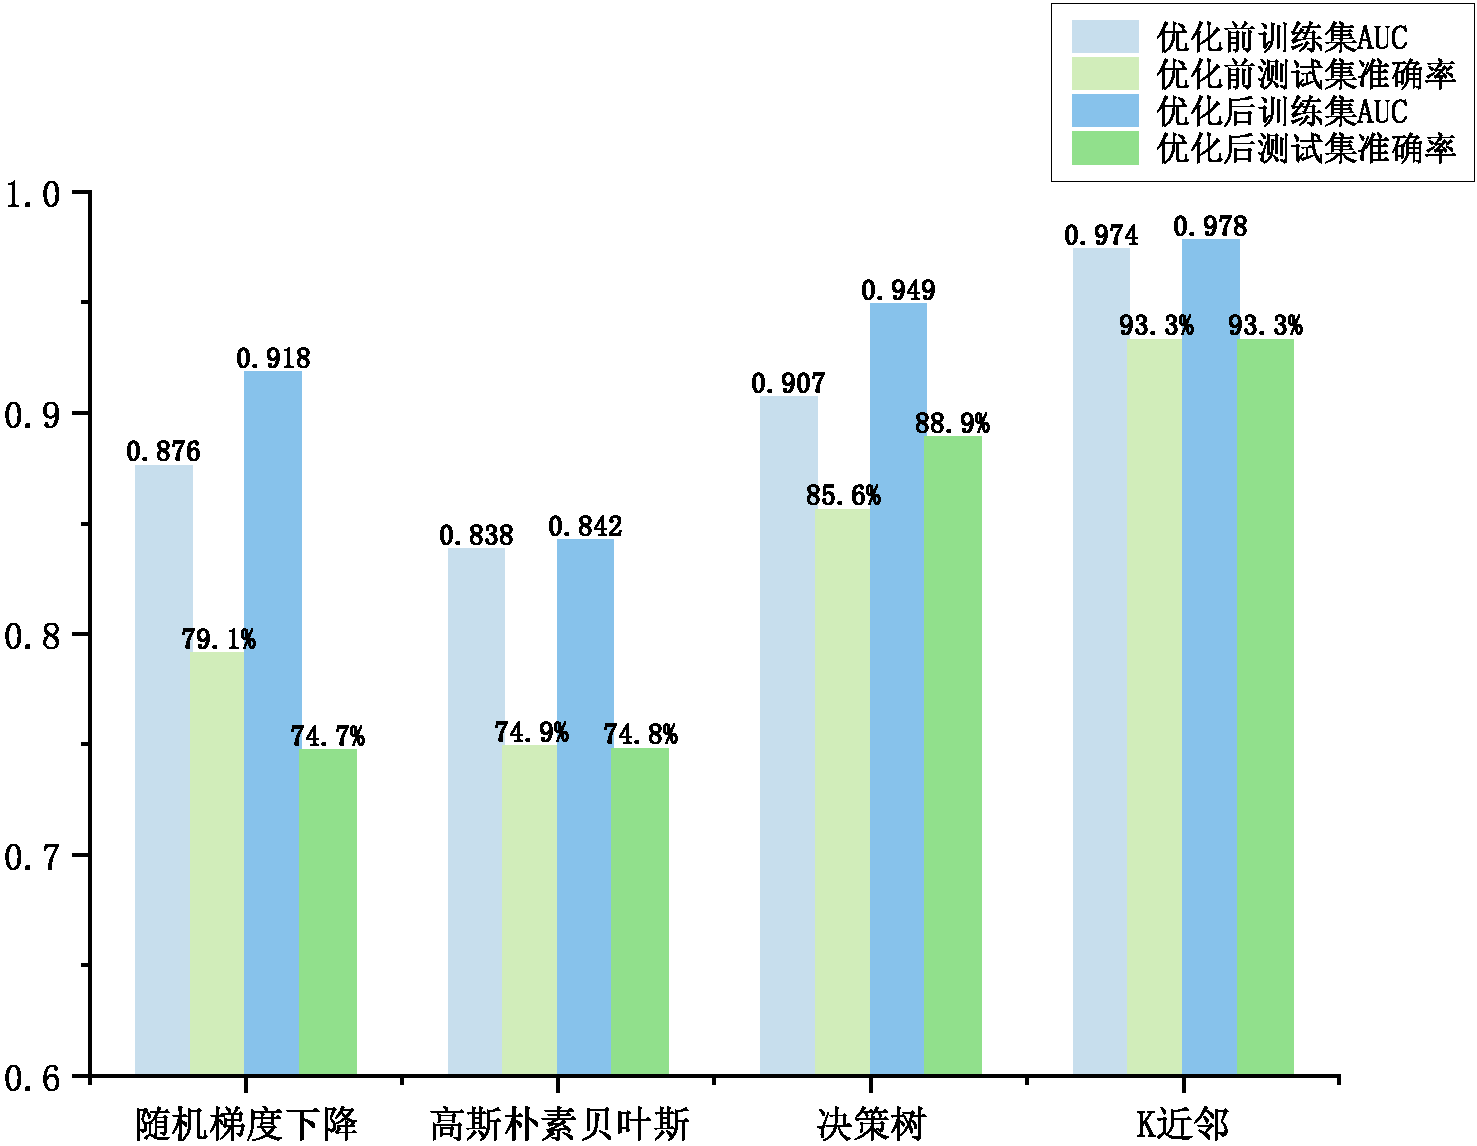
\includegraphics[width=6.5cm]{results/contrast_model1}
      }
      \quad
      \subfigure[\label{fig:cmdl2}各模型在超参数优化前后的性能对比]{
      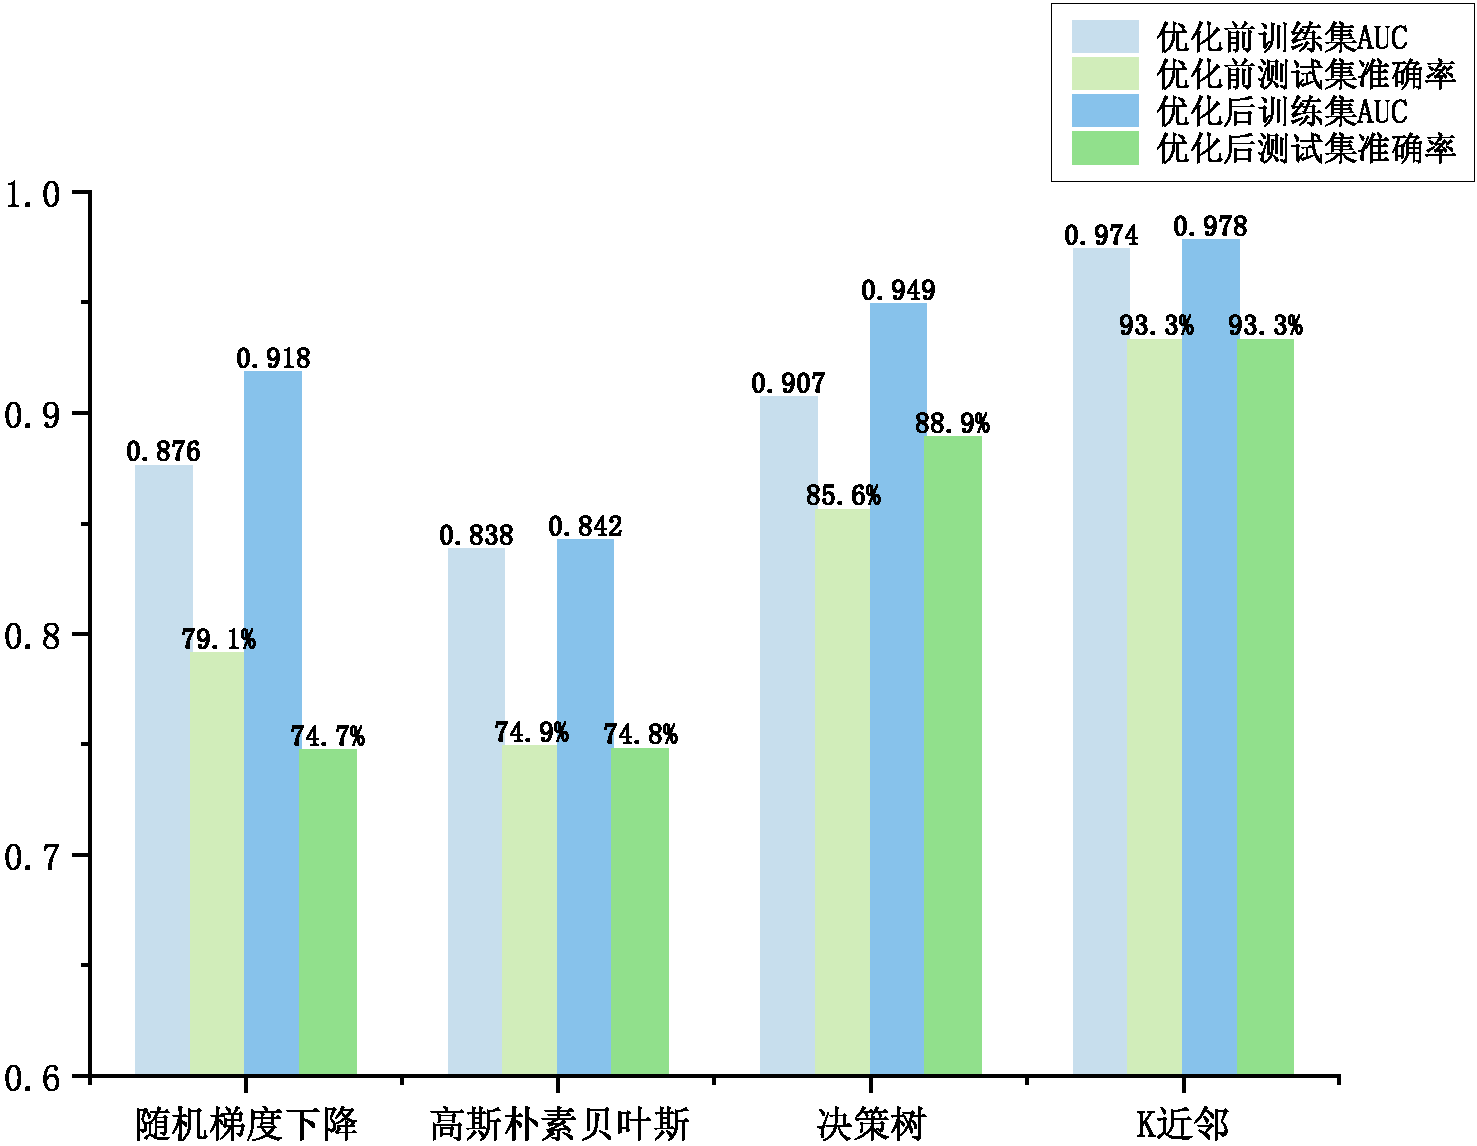
\includegraphics[width=6.5cm]{results/contrast_model2}
      }
      \caption{\label{fig:contrast_model}各模型在超参数优化前后的性能对比}
\end{figure}

从\autoref{fig:contrast_model}展现的数值上看,由于测试集上AUC是作为超参数调优的衡量标准,四种模型的AUC数值按预期有一定的数值提升;但从测试集上的准确率来看,只有DT与KNN算法
延续了上步中较为优秀的性能表现,经由算法得到的模型在测试集上的准确率有一定的提升。这也进一步佐证了上步模型初筛中得到的各项结论。

三、随机森林算法与特征降维

由于集成学习通常会较仅使用单一算法的机器学习具有更好的性能表现,故在此以集成学习的代表性RF算法也进行了PE识别模型的训练,并在此基础上进行了
PPGMTFS中各属性的贡献度分析与PPGMTFS的特征降维处理。

直接利用默认超参数即可以训练得到PE识别的RF模型\cite{scikit-learn}。数值结果表现,RF算法训练得到的模型在训练集与测试集上均有着优秀的表现,
其在训练集上的AUC面积为0.990,在训练集与测试集上的准确率更是分别达到了95.2\%与97.0\%。
这些数值均高于上步中的任一单算法模型的结果,体现了集成学习的优势。

\begin{figure}[htbp]
      \centering
      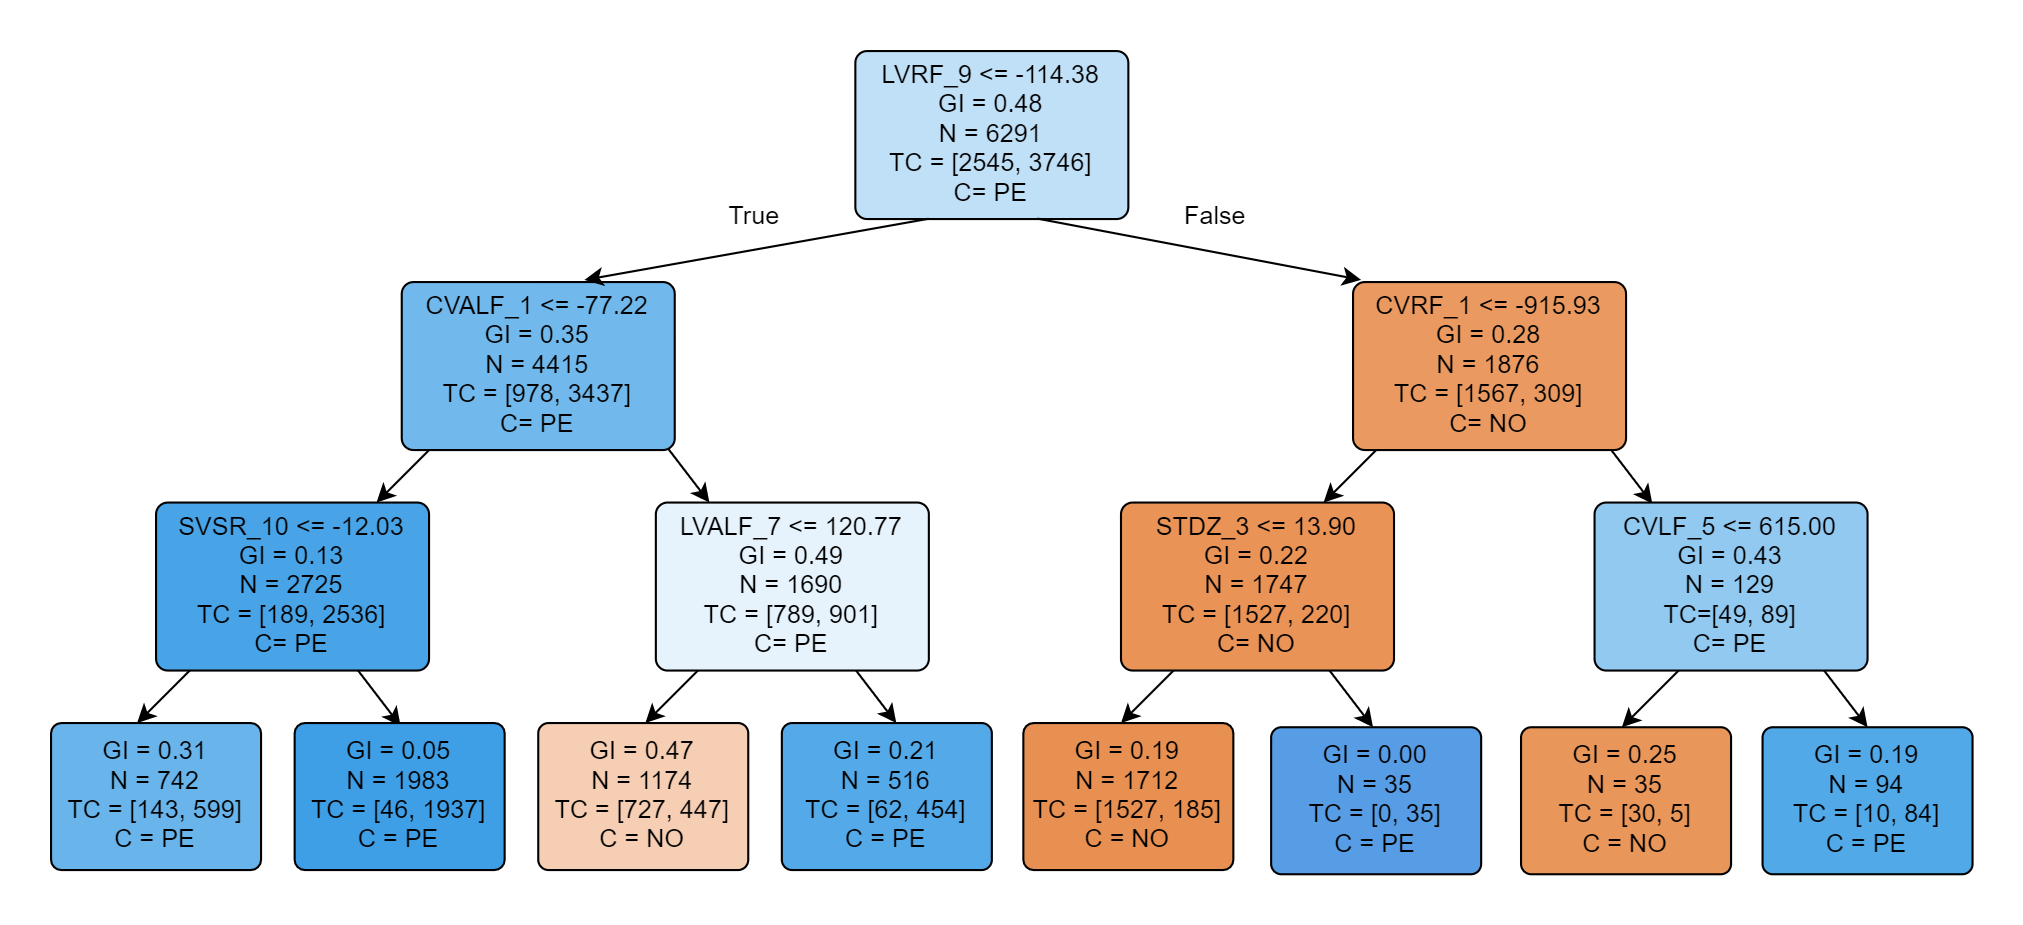
\includegraphics[width=\linewidth]{results/rfdt}
      \caption{\label{fig:dt_clf}由随机森林算法构建得到的决策树示意}
\end{figure}

利用RF算法构成多棵DT形成森林之后,可以得到每棵DT中使用的特征及其相对深度。\autoref{fig:dt_clf}则给出了此RF中一棵具体的DT,其中每个节点均给出用于判断的关键特征及其数值、
GI数值、样本总数N、实际所属类别TC(有无PE的病发)与预测类别,节点的深浅颜色也代表了实际所属类别的比值大小。
对统计RF中所有DT的特征及其相对深度进行统计,可得各特征在RF中的平均深度,该值即为各特征对最终PE识别模型的贡献度,其结果如\autoref{tab:rf_dr_1}。

\begin{center}
      \zihao{-5}
      \begin{longtable}{m{1.5cm}<{\centering}m{2cm}<{\centering}m{2cm}<{\centering}m{2cm}<{\centering}m{2cm}<{\centering}m{2cm}<{\centering}}
            \caption[参与构建随机森林的特征贡献度(部分)]{参与构建随机森林的特征贡献度(部分)}\\
            \label{tab:rf_dr_1}\\
            \topline
            \colorhead \textbf{特征名}&\textbf{贡献度}&\textbf{特征名}&\textbf{贡献度}&\textbf{特征名}&\textbf{贡献度}\\
            \midline
            \endfirsthead
            \caption[]{(续)}\\
            \midline
            \colorhead \textbf{特征名}&\textbf{贡献度}&\textbf{特征名}&\textbf{贡献度}&\textbf{特征名}&\textbf{贡献度}\\
            \midline
            \endhead 
            \midline
            \endfoot
            \bottomline
            \endlastfoot
            \cellcolor{cyan}CVALF\_9                         & \cellcolor{cyan}4.6\%                            & \cellcolor{cyan}LVRF\_9                          & \cellcolor{cyan}3.4\%                            & SVD\_10                          & 3.0\%                            \\
            \cellcolor{cyan}SVAF\_10                         & \cellcolor{cyan}2.5\%                            & \cellcolor{cyan}LVALF\_7                         & \cellcolor{cyan}2.4\%                            & SVAT\_10                         & 2.3\%                            \\
            \cellcolor{cyan}CVRF\_11                         & \cellcolor{cyan}2.1\%                            & \cellcolor{pink}SVAR\_10                         & \cellcolor{pink}1.8\%                            & STDZ\_3                          & 1.6\%                            \\
            \cellcolor{cyan}LVRF\_8                          & \cellcolor{cyan}1.6\%                            & \cellcolor{cyan}LVALF\_6                         & \cellcolor{cyan}1.6\%                            & CVD\_11                          & 1.6\%                            \\
            STDZ\_1                                          & 1.5\%                                            & \cellcolor{cyan}CVALF\_8                         & \cellcolor{cyan}1.5\%                            & SVD\_9                           & 1.4\%                            \\
            \cellcolor{pink}SVAAR\_10                        & \cellcolor{pink}1.4\%                            & \cellcolor{cyan}CVALF\_1                         & \cellcolor{cyan}1.4\%                            & \cellcolor{pink}SVAAR\_8                         & \cellcolor{pink}1.3\%                            \\
            SVD\_8                                           & 1.1\%                                            & \cellcolor{pink}SVAR\_9                          & \cellcolor{pink}1.0\%                            & \cellcolor{cyan}SVAF\_9                          & \cellcolor{cyan}1.0\%                            \\
            \cellcolor{cyan}CVAAF\_1                         & \cellcolor{cyan}1.0\%                            & \cellcolor{cyan}LVLF\_8                          & \cellcolor{cyan}0.9\%                            & SVAT\_8                          & 0.9\%                            \\
            \cellcolor{cyan}CVRF\_1                          & \cellcolor{cyan}0.9\%                            & \cellcolor{cyan}CVAAF\_2                         & \cellcolor{cyan}0.9\%                            & \cellcolor{pink}SVAR\_8                          & \cellcolor{pink}0.8\%                            \\
            \cellcolor{cyan}SVAF\_2                          & \cellcolor{cyan}0.8\%                            & \cellcolor{pink}CVRR\_11                         & \cellcolor{pink}0.8\%                            & \cellcolor{cyan}LVRF\_1                          & \cellcolor{cyan}0.7\%                            \\
            \cellcolor{pink}SVSR\_7                          & \cellcolor{pink}0.7\%                            & \cellcolor{cyan}CVRF\_3                          & \cellcolor{cyan}0.7\%                            & \cellcolor{pink}CVALR\_10                        & \cellcolor{pink}0.7\%                            \\
            \cellcolor{cyan}CVALF\_7                         & \cellcolor{cyan}0.7\%                            & \cellcolor{pink}CVAAR\_5                         & \cellcolor{pink}0.7\%                            & \cellcolor{cyan}LVRF\_2                          & \cellcolor{cyan}0.6\%                           
      \end{longtable}
\end{center}
\vspace{-0.8cm}

\autoref{tab:rf_dr_1}列举了PPGMTFS的286个时域特征对RF累计贡献度排名靠前的36个特征,这些特征的累计贡献度为51.9\%。其中,基于PPG上升支的特征使用了粉红色背景填充,基于PPG下降支的特征为蓝色背景填充;特征名后的数字下标代表了
特征所对应的PPG位置,越靠近峰值的位置下标值越小。若以\autoref{tab:rf_dr_1}中的贡献度最大的特征CVALF\_9(4.6\%)为基准,可以得到所有特征对RF模型的相对贡献度如\autoref{fig:rf_importance_pulse}所示所示。

\begin{figure}[htbp]
      \centering
      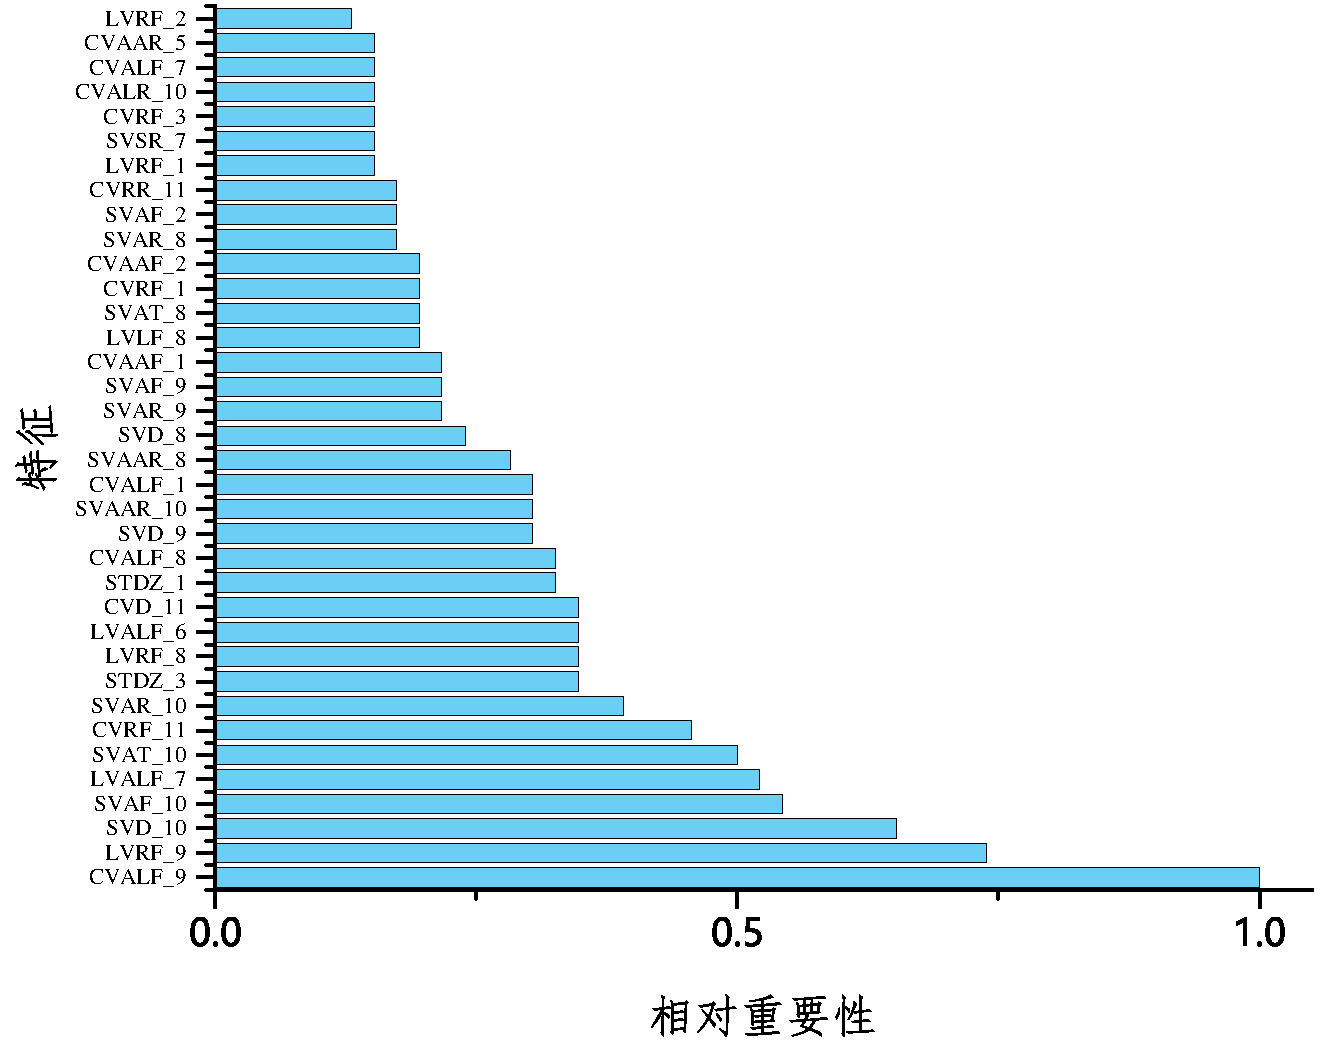
\includegraphics[width=0.6\linewidth]{results/rf_ip_pulse_0.52}
      \caption[各特征对随机森林的相对贡献度(局部)]{\label{fig:rf_importance_pulse}各特征对随机森林的相对贡献度(局部)}
\end{figure}

另一方面,在获取各特征对最终PE识别模型的贡献度后,可按照贡献度按从高到低的顺序进行特征筛选。
本研究按10\%为梯度,完成了从贡献度10\%到90\%的特征筛选过程,基于每个梯度下筛选出的特征子集也使用RF算法
训练了PE识别模型,该过程中各项具体数值结果如\autoref{tab:rf_dr_2}所示。

\begin{center}
      \zihao{-5}
      \begin{longtable}{m{2cm}<{\centering}m{1.3cm}<{\centering}m{1.3cm}<{\centering}m{1.6cm}<{\centering}m{1cm}<{\centering}m{1cm}<{\centering}m{1cm}<{\centering}m{1cm}<{\centering}m{1cm}<{\centering}}
            \caption{随机森林对脉搏波特征降维效果}\\
            \label{tab:rf_dr_2}\\
            \topline
            \colorhead \multicolumn{3}{c}{\textbf{随机森林特征输入}}              &  &  & \multicolumn{4}{c}{\textbf{测试集}}                                          \\
            \colorhead \textbf{贡献度比例} & \textbf{特征数量} & \textbf{数量比例} & \multirow{-2}{*}{\textbf{训练时间}}  & \multirow{-2}{*}{\textbf{AUC}}   & \textbf{精确率} & \textbf{召回率} & \textbf{F1值} & \textbf{准确率} \\
            \midline
            \endfirsthead
            \caption[]{(续)}\\
            \midline
            \colorhead \multicolumn{3}{c}{\textbf{随机森林特征输入}}              &  &  & \multicolumn{4}{c}{\textbf{测试集}}                                          \\
            \colorhead \textbf{贡献度比例} & \textbf{特征数量} & \textbf{数量比例} & \multirow{-2}{*}{\textbf{训练时间}}  & \multirow{-2}{*}{\textbf{AUC}}   & \textbf{精确率} & \textbf{召回率} & \textbf{F1值} & \textbf{准确率} \\
            \midline
            \endhead 
            \midline
            \endfoot
            \bottomline
            \endlastfoot
            \colorrowa 10.0\%         & 3             & 1.0\%         & 5.31     & 0.931      & 89.3\%       & 86.8\%       & 88.0\%       & 86.0\%       \\
            \colorrowc 20.0\%         & 7             & 2.4\%         & 7.82     & 0.961      & 94.5\%       & 90.1\%       & 92.3\%       & 91.0\%       \\
            \colorrowa 30.0\%         & 13            & 4.5\%         & 9.79     & 0.987      & 97.4\%       & 96.4\%       & 96.9\%       & 96.3\%       \\
            \colorrowc 40.0\%         & 21            & 7.3\%         & 11.90    & 0.993      & 97.7\%       & 96.8\%       & 97.3\%       & 96.8\%       \\
            \colorrowa 50.0\%         & 34            & 11.9\%        & 15.17    & 0.993      & 97.8\%       & 97.0\%       & 97.4\%       & 97.0\%       \\
            \colorrowc 60.0\%         & 51            & 17.8\%        & 20.91    & 0.994      & 98.3\%       & 97.1\%       & 97.7\%       & 97.3\%       \\
            \colorrowa 70.0\%         & 74            & 25.9\%        & 23.67    & 0.993      & 98.1\%       & 97.5\%       & 97.8\%       & 97.4\%       \\
            \colorrowc 80.0\%         & 108           & 37.8\%        & 29.33    & 0.993      & 97.7\%       & 97.2\%       & 97.5\%       & 97.0\%       \\
            \colorrowa 90.0\%         & 162           & 56.6\%        & 38.11    & 0.991      & 98.1\%       & 97.3\%       & 97.8\%       & 97.3\%       \\
            \colorrowc 100.0\%        & 286           & 100.0\%       & 41.30    & 0.990      & 98.0\%       & 97.0\%       & 97.5\%       & 97.0\%       \\
      \end{longtable}
\end{center}
\vspace{-0.8cm}

分析上述特征降维处理过程中\autoref{tab:rf_dr_2}、\autoref{tab:rf_dr_2}与\autoref{fig:rf_importance_pulse},可以得到以下结论:

1、PPGMTFS包含了与PE相关性较强的特征。从数值上来看,特征集的286个特征的平均贡献度为0.34\%,而对由RF算法得到的贡献度最高的单特征CVALF\_9的贡献度为4.6\%,该值为平均值的13.5倍。
而从\autoref{tab:rf_dr_2}的特征贡献度来看,PPGMTFS的286个特征中与PE相关性较强的特征较少,存在着无PE相关性较低的冗余特征。在保留原始特征集90\%的贡献度的条件下,就可以
在几乎不损失模型预测能力的条件下排除
\clearpage
\noindent
约43.4\%的无关特征。

2、从\autoref{tab:rf_dr_1}中特征种类来看,与PPG下降支相关的特征要远多于PPG上升支的特征,这可能与PPG下降支是血液回流过程的反应、下降支包含了更多的血液循环中细节信息的事实有关。同时,\autoref{tab:rf_dr_1}中
贡献度较高的特征主要集中在前端(1-3)与尾端(8-10),这说明PPG下降支的前端与尾端可能包含了更多与PE相关的生理学信息。而从这些特征计算过程中对应的基准点确定策略来看,
左视类指标相较中视类指标与分层类指标也更少,这说明了较另外两种策略而言,左视类指标对下降支的表征效果最差。

3、从\autoref{tab:rf_dr_2}的特征降维过程来看,随着特征数量的减少,RF模型的训练速度大大加快,新生成的RF模型在训练集与测试集上均出现了性能小幅提高再下降的整体趋势,
模型最佳性能出现在贡献度60\%-70\%之间。这说明筛选刚开始进行时排除了无关冗余特征,从而使模型性能得到了提升;而随着筛选的进行,对模型生成贡献度较大的特征数量的也在减少,并使最后模型的性能降低。

\subsection{基于被试的研究}
SR基于孕妇的一段时间内采集得到的所有 PPG 波形包含了可以识别区分PE的全部信息这一猜想,将单个被试的所有PPG波形作为一个整体进行分析处理。
SR使用了第四章提及的对被试分层抽样的数据作为训练集与测试集,在此基础上,使用了前文研究中综合性能较好的KNN、DT与RF等三种算法进行PE识别模型的训练。

\autoref{tab:model_screen2}给出了KNN、DT与RF等三种算法训练得到的模型的具体表现,其中,训练集上的AUC数值是在进行5层交叉验证后得到的。

\begin{center}
      \zihao{-5}
      \begin{longtable}{m{2cm}<{\centering}m{1.1cm}<{\centering}m{1cm}<{\centering}m{1cm}<{\centering}m{1cm}<{\centering}m{1cm}<{\centering}m{1cm}<{\centering}m{1cm}<{\centering}m{1cm}<{\centering}m{1cm}<{\centering}m{1cm}<{\centering}}
            \caption{几种机器学习模型在被试人员分层抽样的数据集上的表现}\\
            \label{tab:model_screen2}\\
            \topline
            \colorhead &  & \multicolumn{5}{c}{\textbf{训练集}} & \multicolumn{4}{c}{\textbf{验证集}}                                                                                                                                                                                                      \\
            \colorhead \multirow{-2}{*}{\textbf{模型类型}} & \multirow{-2}{*}{\textbf{训练时间}}  &  \textbf{精确率} &  \textbf{召回率} &  \textbf{F1值} &  \textbf{准确率} &  \textbf{AUC}  &  \textbf{精确率} &  \textbf{召回率} &  \textbf{F1值} &  \textbf{准确率}    \\
            \midline
            \endfirsthead
            \caption[]{(续)}\\
            \midline
            \colorhead &  & \multicolumn{5}{c}{\textbf{训练集}} & \multicolumn{4}{c}{\textbf{验证集}}                                                                                                                                                                                                      \\
            \colorhead \multirow{-2}{*}{\textbf{模型类型}} & \multirow{-2}{*}{\textbf{训练时间}}  &  \textbf{精确率} &  \textbf{召回率} &  \textbf{F1值} &  \textbf{准确率} &  \textbf{AUC}  &  \textbf{精确率} &  \textbf{召回率} &  \textbf{F1值} &  \textbf{准确率}    \\
            \midline
            \endhead 
            \midline
            \endfoot
            \bottomline
            \endlastfoot
            \colorrowa K近邻算法      &   4.08 s   & 88.0\% & 76.0\% &81.6\% & 80.0\% & 0.870 & 81.5\% & 85.6\% & 83.5\% & 78.3\% \\
            \colorrowc 决策树算法      &   1.44 s  & 84.0\% & 80.9\% & 82.4\% & 79.8\% & 0.862 & 69.0\% & 86.1\% & 76.6\% & 66.3\% \\
            \colorrowa 随机森林算法      &   50.03 s  & 90.6\% & 80.6\% & 85.3\% & 83.8\% & 0.929 & 79.5\% & 90.9\% & 84.8\% & 79.1\% \\
      \end{longtable}
\end{center}
\vspace{-0.8cm}

从\autoref{tab:model_screen2}可以发现,由RF与KNN算法训练所得的模型的性能接近,在测试集上F1值可达到83\%以上,准确率也在78\%以上;而DT算法生成的模型性能最差,其F1值与准确率分别仅为76.6\%与66.3\%。
将\autoref{tab:model_screen2}的数值结果与此前的\autoref{tab:model_screen}及\autoref{tab:rf_dr_2}中结果对比可得,相较PR的方式,在SR方式下,KNN、DT与RF等三种算法在训练集与测试集上均出现了
较为明显的性能下降,在测试集上性能下降得尤为明显。这一现象可能与测试集中的被试的任何PPG波形从未在训练集中出现有关。

注意到\autoref{tab:model_screen2}中评价模型的性能的各指标仍是按照单个PPG波形统计的,并不能完全反应SR方式下被试PPG波形与PE之间关系。
在\autoref{tab:model_screen2}测试集中,将反应单个PPG波形的识别结果重新按被试统计可得到\autoref{tab:model_detail}。
\autoref{tab:model_detail}额外统计了每名被试所对应的PPG波形总数与由预测模型识别判断为PE的PPG波形数目,预测比例一栏为这两个数值之比,
而每名被试所对应的真实PE状态也在\autoref{tab:model_detail}进行了标记。

\begin{center}
      \zihao{-5}
      \begin{longtable}{m{1.2cm}<{\centering}m{1cm}<{\centering}m{1.2cm}<{\centering}m{1.5cm}<{\centering}m{1.5cm}<{\centering}m{1.5cm}<{\centering}m{1.5cm}<{\centering}m{1.5cm}<{\centering}m{1.5cm}<{\centering}m{1cm}<{\centering}}
            \caption{几种机器学习模型按被试统计后的性能表现}\\
            \label{tab:model_detail}\\
            \topline
            \colorhead  &  & & \multicolumn{2}{c}{\textbf{K近邻算法}} & \multicolumn{2}{c}{\textbf{决策树}} & \multicolumn{2}{c}{\textbf{随机森林}}  \\
            \colorhead \multirow{-2}{*}{\textbf{被试孕妇}}  &     \multirow{-2}{*}{\textbf{PE状态}} &   \multirow{-2}{*}{\textbf{波形总数}}   & \textbf{预测数目}     & \textbf{预测比例}       & \textbf{预测数目}     & \textbf{预测比例}       & \textbf{预测数目}     & \textbf{预测比例}             \\
            \midline
            \endfirsthead
            \caption[]{(续)}\\
            \midline
            \colorhead  &  & & \multicolumn{2}{c}{\textbf{K近邻算法}} & \multicolumn{2}{c}{\textbf{决策树}} & \multicolumn{2}{c}{\textbf{随机森林}}  \\
            \colorhead \multirow{-2}{*}{\textbf{被试孕妇}}  &     \multirow{-2}{*}{\textbf{PE状态}} &   \multirow{-2}{*}{\textbf{波形总数}}   & \textbf{预测数目}     & \textbf{预测比例}       & \textbf{预测数目}     & \textbf{预测比例}       & \textbf{预测数目}     & \textbf{预测比例}             \\
            \midline
            \endhead 
            \midline
            \endfoot
            \bottomline
            \endlastfoot
            \colorrowa cmf       & 0           & 88                    & 54         & 61.4\%     & 85         & 96.6\%     & 53         & 60.2\%                                                                            \\
            \colorrowc lxx       & 0           & 63                    & 32         & 50.8\%     & 53         & 84.1\%     & 34         & 54.0\%                                                                            \\
            \colorrowa shs       & 0           & 112                   & 37         & 33.0\%     & 105        & 93.8\%     & 55         & 49.1\%                                                                            \\
            \colorrowc sxh       & 0           & 95                    & 27         & 28.4\%     & 64         & 67.4\%     & 21         & 22.1\%                                                                            \\
            \colorrowa wdq       & 0           & 36                    & 0          & 0.0\%      & 0          & 0.0\%      & 0          & 0.0\%                                                                             \\
            \colorrowc wsj       & 0           & 78                    & 0          & 0.0\%      & 2          & 2.6\%      & 0          & 0.0\%                                                                             \\
            \colorrowa ygy       & 0           & 75                    & 40         & 53.3\%     & 70         & 93.3\%     & 67         & 89.3\%                                                                            \\
            \colorrowc gmn       & 1           & 139                   & 106        & 76.3\%     & 135        & 97.1\%     & 109        & 78.4\%                                                                            \\
            \colorrowa ty        & 1           & 98                    & 97         & 99.0\%     & 97         & 99.0\%     & 97         & 99.0\%                                                                            \\
            \colorrowc wjh       & 1           & 86                    & 86         & 100.0\%    & 86         & 100.0\%    & 86         & 100.0\%                                                                           \\
            \colorrowa xjf       & 1           & 106                   & 23         & 21.7\%     & 59         & 55.7\%     & 87         & 82.1\%                                                                            \\
            \colorrowc ywy       & 1           & 111                   & 110        & 99.1\%     & 111        & 100.0\%    & 111        & 100.0\%                                                                           \\
            \colorrowa yxl       & 1           & 110                   & 110        & 100.0\%    & 108        & 98.2\%     & 110        & 100.0\%                                                                           \\
            \colorrowc zdq       & 1           & 89                    & 81         & 91.0\%     & 84         & 94.4\%     & 82         & 92.1\%                                                                            \\
            \colorrowa zl        & 1           & 152                   & 137        & 90.1\%     & 75         & 49.3\%     & 120        & 78.9\%                                                                            \\
            \colorrowc zyy       & 1           & 89                    & 89         & 100.0\%    & 89         & 100.0\%    & 89         & 100.0\%                                                                            \\    
      \end{longtable}
\end{center}
\vspace{-0.8cm}

若将\autoref{tab:model_detail}中经由各模型对应的预测比例作为判断识别PE的依据,则对PE的识别分析可以转换为寻找
能将这些预测比例进行分割的最佳阈值。\autoref{fig:model_detail}展示了测试集每名被试的预测比例所对应的散点图,并进一步可到与经由每种算法得到的预测比例在PE识别问题上的ROC曲线,如\autoref{fig:model_roc}所示。
此过程中涉及的各算法最佳阈值及最佳阈值下的CM、准确率与AUC数值结果如如\autoref{tab:cm_on_best}所示。
\begin{figure}[htbp]
      \centering
      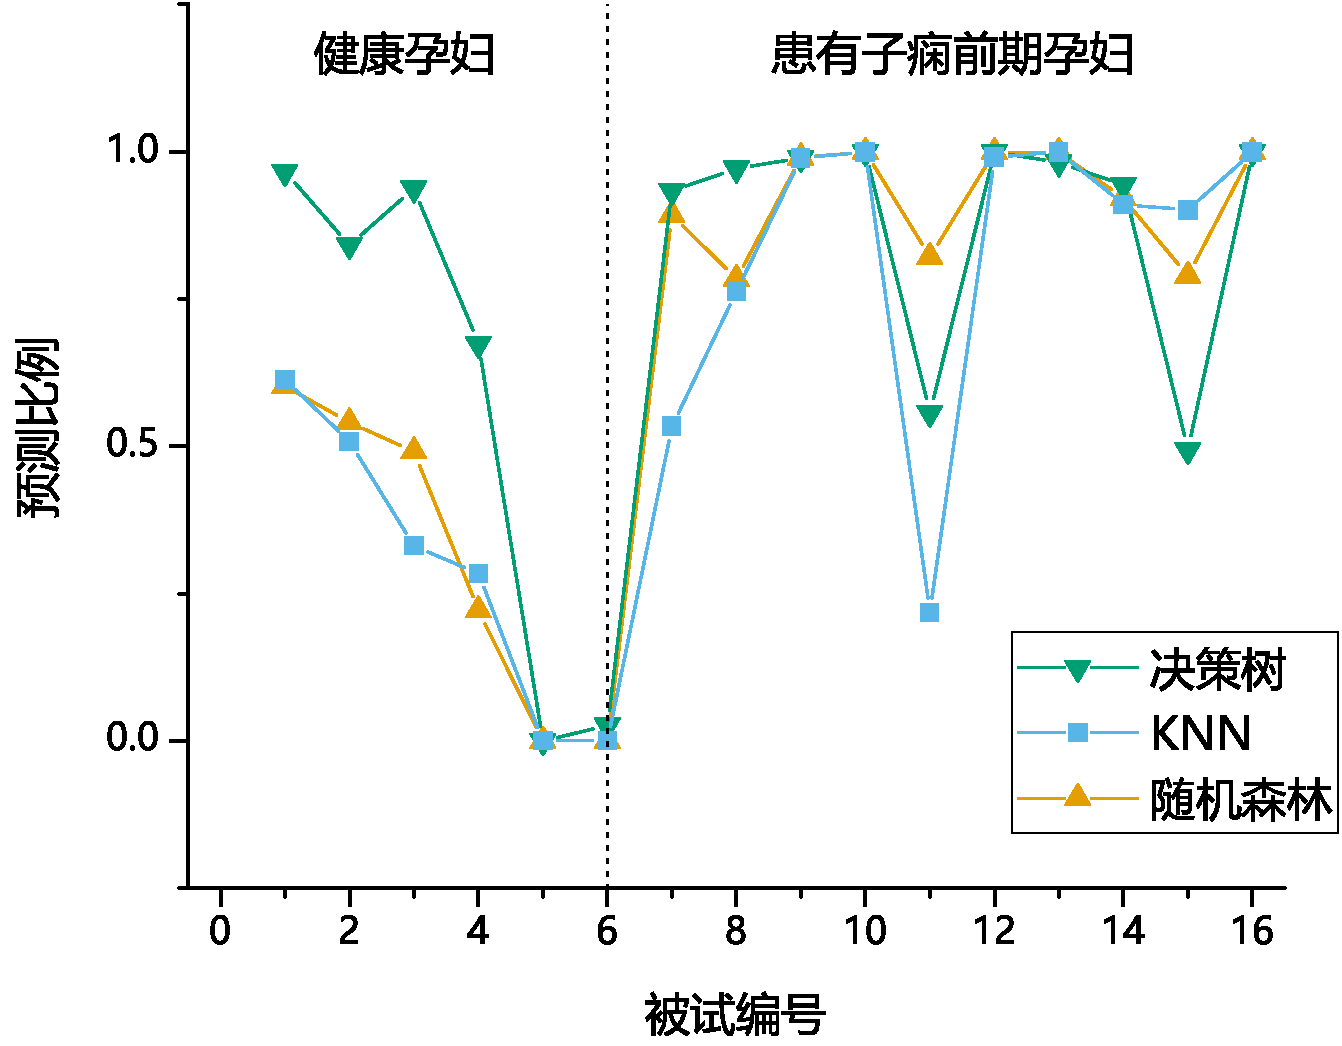
\includegraphics[width=.55\linewidth]{results/detail}
      \caption[基于三种算法得到的子痫前期预测比例散点图]{\label{fig:model_detail}基于三种算法得到的子痫前期预测比例散点图}
\end{figure}

\begin{figure}[htbp]
      \centering
      \includegraphics[width=.55\linewidth]{results/roc}
      \caption[由子痫前期预测比例得到的ROC曲线]{\label{fig:model_roc}由子痫前期预测比例得到的ROC曲线}
\end{figure}
\vspace{-1cm}

\begin{center}
      \zihao{-5}
      % \setlength{\belowcaptionskip}{-0.5cm} 
      \begin{longtable}{m{2.8cm}<{\centering}m{2cm}<{\centering}m{1.5cm}<{\centering}m{1.8cm}<{\centering}m{1.8cm}<{\centering}}
            \caption{三种模型在最佳分割阈值下的混淆矩阵}\\
            \label{tab:cm_on_best}\\
            \topline
            \colorhead \textbf{机器学习算法}&\textbf{最佳阈值}&\textbf{混淆矩阵}&\textbf{准确率}&\textbf{AUC}\\
            \midline
            \endfirsthead
            \caption[]{(续)}\\ 
            \topline
            \colorhead \textbf{机器学习算法}&\textbf{最佳阈值}&\textbf{混淆矩阵}&\textbf{准确率}&\textbf{AUC}\\
            \midline
            \endhead 
            \midline
            \endfoot
            \bottomline
            \endlastfoot
            \colorrowa DT       & 0.969    &     $\left[ \begin{array}{cc} 6 & 3 \\ 0 & 7 \end{array} \right]$  & 81.3\% & 0.825  \\
            \colorrowc KNN       & 0.907     &     $\left[ \begin{array}{cc} 6 & 3 \\ 0 & 7 \end{array} \right]$  & 81.3\% & 0.921 \\
            \colorrowa RF     & 0.688    &     $\left[ \begin{array}{cc} 9 & 0 \\ 1 & 6 \end{array} \right]$  & 93.8\% & 0.952  \\
      \end{longtable}
\end{center}
\vspace{-1.4cm}

从上述研究结果中可以发现,在SR方式下,借助由ML算法得到的预测比例数值可以较好的识别PE。通过AUC与ROC分析,在三种构建模型的算法中,RF算法有着最佳的分类效果,其AUC数值最大(0.952)、识别准确率最高
(93.8\%),RF算法识别为假阴性的数目(0)也少于其他两种模型(均为3)。而从最佳分割阈值来看,DT与KNN算法的预测比例分割阈值(0.969与0.907)过于接近100\%,有泛化能力不足的潜在风险,而RF模型的分割阈值(0.688)则相对适中。

\section{基于PPG采样值时域特征集的机器学习分析}
本小节基于第四章提出的PPG采样值时域特征集(PPGSTFS),围绕基于PPG波形(PR)与基于被试(SR)等两个研究方向,利用多种ML算法,进行了PE识别分析模型的相关研究。
注意到PPGSTFS中可能需要对PPG波形进行对齐处理,本小节按第四章中介绍过重采样策略(RS)与补齐策略(CS)分别进行了处理。

\subsection{基于PPG波形的研究}
PR将单个PPG波形作为分析识别PE的最小分析对象,认为PPG的波形是孕妇PE病发状态的稳定“表达”,单个PPG波形包含了可以识别区分PE的全部信息。
PR使用了第四章提及的对波形分层抽样的数据作为训练集与测试集。在此基础上,进行了ML算法初筛、算法超参数优化及特征贡献度分析等研究工作。

一、模型初筛与调优

模型初筛选用此前综合性能较好的DT、KNN及RF等三种算法,这三种算法在全局最优超参数下的综合表现如\autoref{tab:model_screen3}所示,其中各模型训练集的统计结果是经5层交叉验证处理后得到的。
\begin{center}
      \zihao{-5}
      \begin{longtable}{m{1.2cm}<{\centering}m{1.2cm}<{\centering}m{1.2cm}<{\centering}m{0.9cm}<{\centering}m{0.9cm}<{\centering}m{0.9cm}<{\centering}m{0.9cm}<{\centering}m{0.9cm}<{\centering}m{0.9cm}<{\centering}m{0.9cm}<{\centering}m{0.9cm}<{\centering}m{0.9cm}<{\centering}}
            \caption{基于脉搏波原始采样点的识别模型的初筛结果}\\
            \label{tab:model_screen3}\\
            \topline
            \colorhead       & \multicolumn{1}{c}{}   & \multicolumn{1}{c}{}  & \multicolumn{5}{c}{\textbf{训练集(5层交叉验证)}}   & \multicolumn{4}{c}{\textbf{验证集}}     \\
            \colorhead \multirow{-2}{*}{\textbf{处理方式}}  & \multirow{-2}{*}{\textbf{模型类型}} & \multirow{-2}{*}{\textbf{训练时间}} & \textbf{精确率} & \textbf{召回率}& \textbf{F1值} & \textbf{准确率}& \textbf{AUC} & \textbf{精确率} & \textbf{召回率} & \textbf{F1值}& \textbf{准确率} \\
            \midline
            \endfirsthead
            \caption[]{(续)}\\
            \midline
            \colorhead       & \multicolumn{1}{c}{}   & \multicolumn{1}{c}{}  & \multicolumn{5}{c}{\textbf{训练集(5层交叉验证)}}   & \multicolumn{4}{c}{\textbf{验证集}}                                                                                                                                                                                                    \\
            \colorhead \multirow{-2}{*}{\textbf{处理方式}}  & \multirow{-2}{*}{\textbf{模型类型}} & \multirow{-2}{*}{\textbf{训练时间}} & \textbf{精确率} & \textbf{召回率}& \textbf{F1值} & \textbf{准确率}& \textbf{AUC} & \textbf{精确率} & \textbf{召回率} & \textbf{F1值}& \textbf{准确率} \\
            \midline
            \endhead 
            \midline
            \endfoot
            \bottomline
            \endlastfoot
            \colorrowa CS & DT      & 4.13    & 83.9\%  & 88.6\%  & 86.1\% & 83.0\% & 0.914   & 86.6\%  & 90.9\%  & 88.7\% & 86.2\% \\
            \colorrowc CS & KNN     & 2.81     & 93.4\%  & 90.0\%  & 91.4\% & 90.0\%   & 0.967  & 94.5\%   & 90.7\%   & 92.6\% & 91.4\% \\
            \colorrowa CS & RF    & 23.23   & 93.3\%  & 92.8\% & 93.0\% & 91.7\%  & 0.977 & 94.8\% & 94.5\%   & 94.6\% & 93.6\% \\
            \colorrowc RS & DT     & 6.77   & 85.6\%  & 85.2\%  & 85.4\% & 82.6\% & 0.902    & 88.3\%  & 84.1\%  & 86.2\% & 83.9\% \\
            \colorrowa RS & KNN     & 3.90    & 91.5\%  & 89.5\%  & 90.5\% & 88.8\%   & 0.957  & 94.2\%   & 91.2\%   & 92.9\% & 91.6\% \\
            \colorrowc RS & RF    & 51.57    & 91.4\%  & 91.9\% & 91.6\% & 90.0\%  & 0.967  & 93.4\% & 94.0\%   & 93.7\% & 92.5\% \\
      \end{longtable}
\end{center}
\vspace{-0.8cm}

从\autoref{tab:model_screen3}中可以得到以下结论:

1、从模型的训练时间方面来看,使用KNN算法构建模型的速度最快,而使用RF算法速度最慢,这一结果也与各算法的时间复杂度一致。

2、从模型在测试集上的表现来看,按CS与IS对PPG进行对齐后,由三种算法得到的模型均能对测试集数据进行较好的学习,各模型的AUC数值均超过了0.900,其中RF模型的AUC数值更是在0.967以上。
而从精度-召回率权衡方面来看,KNN与RF算法明显优于DT算法,这两种算法构建得到的模型的精确率、召回率及F1数值几乎全部在 90.0\% 以上(只有RS下,使用KNN算法得到的模型的召回率为89.5\%)。

3、从模型在验证集上的泛化能力方面来看,KNN与RF算法也明显优于DT算法。就准确率而言,由KNN与RF算法得到的模型可达到91\%以上,而由DT算法得到的模型准确率则不足87\%。
在精度-召回率权衡上,KNN与RF算法也明显优于DT算法,前两种算法训练得到的模型的精确率、召回率及F1等数值均在90.0\%以上,均明显高于DT算法得到的模型表现。

4、综合2与3中结论,可以得到RF算法的综合性能表现最好,KNN算法次之,DT算法表现较差,这进一步验证了集成学习算法较单一算法在训练模型时具有性能优势。

5、横向对比\autoref{tab:model_screen3}中RS与CS等两种对齐PPG波形的策略,使用CS会各模型在构建速度、训练集AUC及模型整体准确率、精确率等方面均略微优于使用RS的对应结果。
 
二、特征贡献度分析

与上小节中处理类似,在PPGTSFS上使用RF算法构建模型后,同样可以得到特征集中各特征对最终模型的贡献度,也即
原始PPG中不同位置上的采样点对模型的贡献度。由于对这些原始采样点进行降维处理无实际意义,本部分未进行相应的降维分析与处理工作。

按CS与RS对PPG对齐处理后,统计各采样点的在生成的RF中的平均深度后,得到两种策略下各采样点的贡献度如\autoref{fig:rf_imp2}所示。
为直观显现各采样点贡献度与PPG波形的对应关系,\autoref{fig:rf_imp2}也同时绘制了在两种策略下的“平均”PPG波形,即所有PPG波形按采样点对齐再计算算术平均值的归一化结果。

\begin{figure}[htbp]
      \centering
      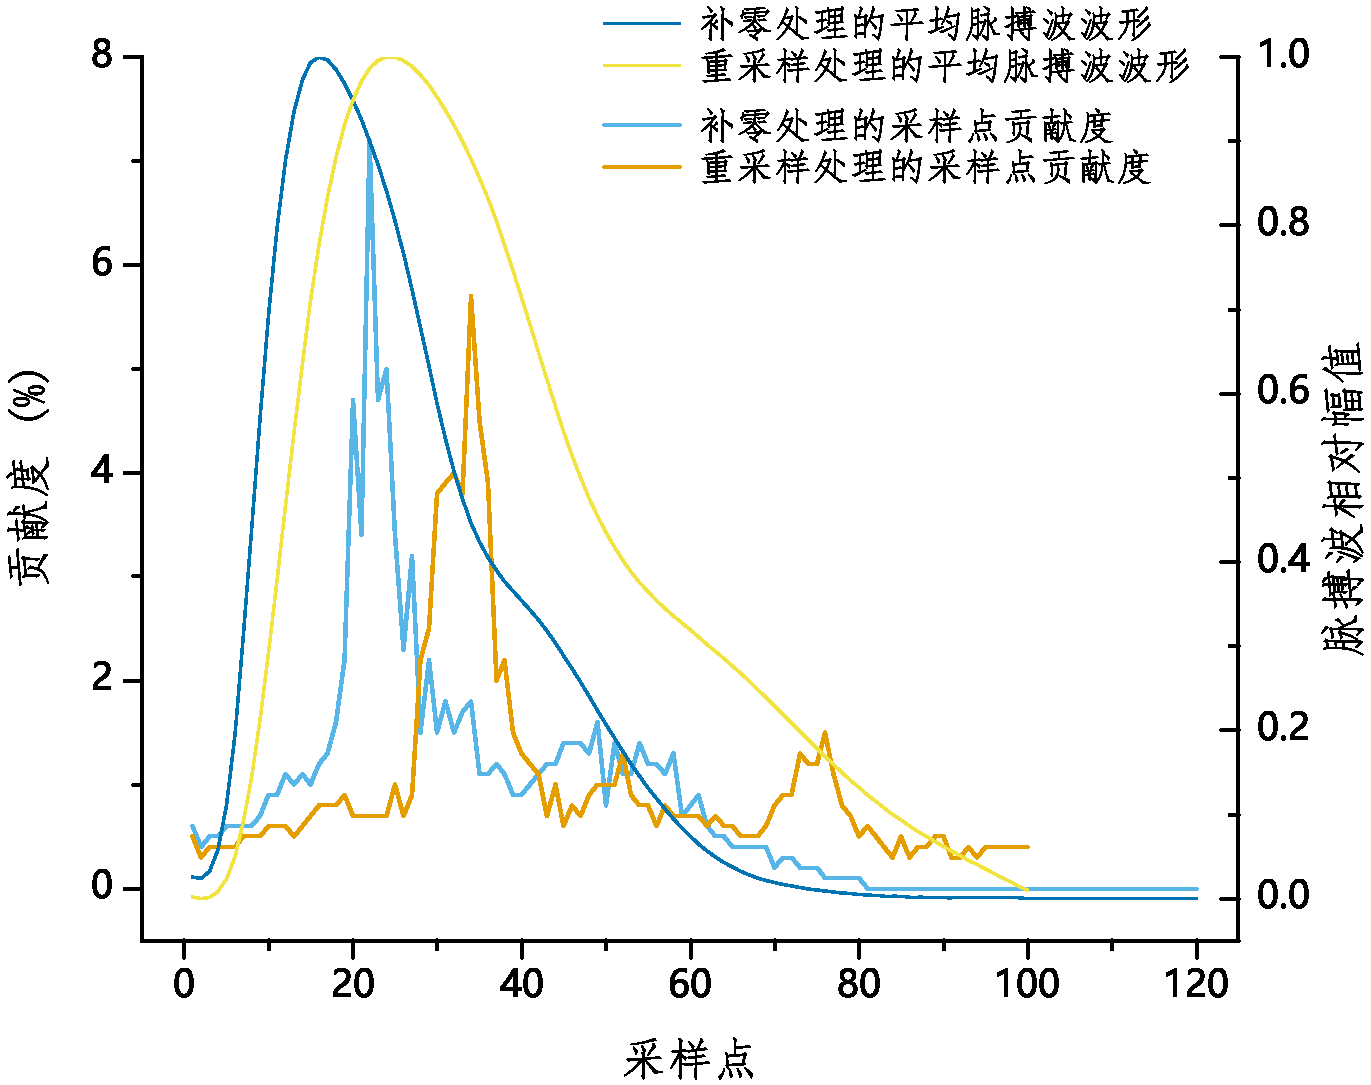
\includegraphics[width=.6\linewidth]{results/rf_imp2}
      \caption{\label{fig:rf_imp2}脉搏波采样点对随机森林的贡献度}
\end{figure}

从\autoref{fig:rf_imp2}可以得到以下结论:

1、两种策略下,各采样点的贡献度分布形态高度相似,均在平均PPG波形的波峰之后出现贡献度的主峰,在平均PPG波形的下降支尾端附近出现第二个次峰。平均PPG波形起点与终点处的采样点较
平均PPG波形波峰附近的采样点贡献度可以忽略不计。

2、对两种处理PPG时长差异的策略而言,尽管CS会得到更多的采样点数(120),但采样点贡献度的具体分布反而更为集中,有效特征点的贡献度数值也更大。
第四章中已经介绍过,本文采集得到的绝大多数PPG波形采样点数均不超过80。而从\autoref{fig:rf_imp2}中也可以观察到,经CS处理后,序号在80以后的采样点贡献度几乎全部为0,也说明这部分采样点几乎没有参与到最终RF模型的构建之中。
但RS而言,重采样后所有PPG波形的采样点数均为100,且不完全为0,这也与\autoref{fig:rf_imp2}中该策略下所有采样点的贡献度均不为0的现象相匹配。

\subsection{基于被试的研究}
SR基于孕妇的一段时间内采集得到的所有 PPG 波形包含了可以识别区分PE的全部信息这一猜想,将单个被试的所有PPG波形作为一个整体进行分析处理。
SR使用了第四章提及的对被试分层抽样的数据作为训练集与测试集,在此基础上,使用了前文研究中综合性能较好的KNN、DT与RF等三种算法进行PE识别模型的训练。

\autoref{tab:model_screen4}给出了由这三种算法训练得到的模型的具体表现,其中,训练集上的AUC数值是在进行5层交叉验证后得到的。

\begin{center}
      \zihao{6}
      \begin{longtable}{m{1.3cm}<{\centering}m{1.3cm}<{\centering}m{1.3cm}<{\centering}m{0.9cm}<{\centering}m{0.9cm}<{\centering}m{0.9cm}<{\centering}m{0.9cm}<{\centering}m{0.9cm}<{\centering}m{0.9cm}<{\centering}m{0.9cm}<{\centering}m{0.9cm}<{\centering}m{0.9cm}<{\centering}}
            \caption{几种机器学习模型在被试人员分层抽样的数据集上的表现}\\
            \label{tab:model_screen4}\\
            \topline
            \colorhead &     &  & \multicolumn{5}{c}{\textbf{训练集}} & \multicolumn{4}{c}{\textbf{验证集}}                                                                                                                                                                                                      \\
            \colorhead \multirow{-2}{*}{\textbf{处理方式}}&\multirow{-2}{*}{\textbf{模型类型}} & \multirow{-2}{*}{\textbf{训练时间}}  &  \textbf{精确率} &  \textbf{召回率} &  \textbf{F1值} &  \textbf{准确率} &  \textbf{AUC}  &  \textbf{精确率} &  \textbf{召回率} &  \textbf{F1值} &  \textbf{准确率}    \\
            \midline
            \endfirsthead
            \caption[]{(续)}\\
            \midline
            \colorhead &     &  & \multicolumn{5}{c}{\textbf{训练集}} & \multicolumn{4}{c}{\textbf{验证集}}                                                                                                                                                                                                      \\
            \colorhead \multirow{-2}{*}{\textbf{处理方式}}&\multirow{-2}{*}{\textbf{模型类型}} & \multirow{-2}{*}{\textbf{训练时间}}  &  \textbf{精确率} &  \textbf{召回率} &  \textbf{F1值} &  \textbf{准确率} &  \textbf{AUC}  &  \textbf{精确率} &  \textbf{召回率} &  \textbf{F1值} &  \textbf{准确率}    \\
            \midline
            \endhead 
            \midline
            \endfoot
            \bottomline
            \endlastfoot
            \colorrowa CS &     KNN      &   3.12 s  & 86.0\% & 73.7\% &79.4\% & 77.6\% & 0.863 & 81.5\% & 85.6\% & 83.5\% & 78.3\% \\
            \colorrowa CS &     DT      &   3.62 s  & 84.0\% & 82.2\% & 83.1\% & 80.5\% & 0.880 & 70.6\% & 84.6\% & 77.0\% & 67.5\% \\
            \colorrowa CS  & RF      &   23.18 s  & 87.0\% & 81.5\% & 84.2\% & 82.1\% & 0.909 & 76.5\% & 86.5\% & 81.2\% & 74.3\% \\
            \colorrowc RS &     KNN      &   2.51 s   & 85.5\% & 76.9\% &81.0\% & 78.9\% & 0.862 & 76.7\% & 80.1\% & 78.4\% & 71.6\% \\
            \colorrowc RS &     DT      &   1.49 s  & 82.7\% & 76.9\% & 79.7\% & 77.1\% & 0.847 & 76.2\% & 88.1\% & 81.7\% & 74.7\% \\
            \colorrowc RS  &  RF     &   36.36 s  & 85.1\% & 77.8\% & 81.2\% & 79.0\% & 0.884 & 78.9\% & 87.6\% & 83.0\% & 77.0\% \\
      \end{longtable}
\end{center}
\vspace{-0.8cm}

从\autoref{tab:model_screen4}中可以得到以下结论:

1、基于SR策略,由KNN、DT与RF等三种算法得到的模型在测试集上的性能并没有表现出明显的差异,在整体准确率、精确率等具体指标上均较为接近。
但与\autoref{tab:model_screen3}中结果相比,三种算法在训练集与测试集上的均出现了较为明显的性能下降,在测试集上性能下降得尤为明显。
这一现象可能与测试集中的被试的任何PPG波形从未在训练集中出现有关。

2、PG时长的对齐策略并不会明显改变\autoref{tab:model_screen4}中各模型在PE识别问题上的性能,各模型在整体准确率、精确率等具体指标上变化幅度很小。

与在PPGMTDS上的处理类似,在\autoref{tab:model_screen4}测试集上,将反应单个PPG波形的识别结果重新按被试统计可得到\autoref{tab:model_detail2}。
\autoref{tab:model_detail2}额外统计了每名被试所对应的PPG波形总数与由预测模型识别判断为PE的PPG波形数目,预测比例一栏为这两个数值之比,
而每名被试所对应的真实PE状态也在\autoref{tab:model_detail2}进行了标记。

\begin{center}
      \zihao{6}
      \begin{longtable}{m{1cm}<{\centering}m{1cm}<{\centering}m{1cm}<{\centering}m{1.5cm}<{\centering}m{2cm}<{\centering}m{1.5cm}<{\centering}m{2cm}<{\centering}m{1.5cm}<{\centering}m{2cm}<{\centering}}
            \caption[几种机器学习模型按被试统计后的性能表现]{几种机器学习模型按被试统计后的性能表现}\\
            \label{tab:model_detail2}\\
            \topline
            \colorhead  &  &  & \multicolumn{2}{c}{\textbf{K近邻算法}} & \multicolumn{2}{c}{\textbf{决策树}} & \multicolumn{2}{c}{\textbf{随机森林}}  \\
            \colorhead \multirow{-2}{*}{\textbf{被试孕妇}}  &     \multirow{-2}{*}{\textbf{PE状态}} &   \multirow{-2}{*}{\textbf{波形总数}}   & \textbf{预测数目}     & \textbf{预测比例}       & \textbf{预测数目}     & \textbf{预测比例}       & \textbf{预测数目}     & \textbf{预测比例}             \\
            \midline
            \endfirsthead
            \caption[]{(续)}\\
            \midline
            \colorhead  &  &  & \multicolumn{2}{c}{\textbf{K近邻算法}} & \multicolumn{2}{c}{\textbf{决策树}} & \multicolumn{2}{c}{\textbf{随机森林}}  \\
            \colorhead \multirow{-2}{*}{\textbf{被试孕妇}}  &     \multirow{-2}{*}{\textbf{PE状态}} &   \multirow{-2}{*}{\textbf{波形总数}}   & \textbf{预测数目}     & \textbf{预测比例}       & \textbf{预测数目}     & \textbf{预测比例}       & \textbf{预测数目}     & \textbf{预测比例}             \\
            \midline
            \endhead 
            \midline
            \endfoot
            \bottomline
            \endlastfoot
            \colorrowa cmf       & 0           & 88                    & 66 / 59         & 75.0\% / 67.0\%     & 75 / 60         & \textbf{85.2\% / 68.2\%}    & 61 / 49         & 69.3\% / 55.7\%                                     \\
            \colorrowc lxx       & 0           & 63                    & 32 / 35         & 50.8\% / 55.6\%    & 50 / 38         & \textbf{79.4\% / 60.3\%}     & 37 / 42         & 58.7\% / 66.7\%                                            \\
            \colorrowa shs       & 0           & 112                   & \textbf{32 / 58}         & \textbf{28.6\% / 51.8\%}     & 102 / 88        & 91.1\% / 78.6\%     & 57 / 47         & 50.1\% / 42.0\%                                                               \\
            \colorrowc sxh       & 0           & 95                    & 31 / 24         & 32.6\% / 25.3\%     & \textbf{52 / 27}         & \textbf{54.7\% / 28.4\%}     & 39 / 21         & \textbf{41.1\% / 22.1\%}                                                               \\
            \colorrowa wdq       & 0           & 36                    & 0 / 0          & 0.0\% / 0.0\%      & 2 / 0          & 5.6\% / 0.0\%      & 0 / 0          & 0.0\% / 0.0\%                                              \\
            \colorrowc wsj       & 0           & 78                    & 0 / 1          & 0.0\% / 0.0\%      & 1 / 0          & 1.3\% / 0.0\%     & 0 / 0          & 0.0\% / 0.0\%                                              \\
            \colorrowa ygy       & 0           & 75                    & 57 / 61         & 76.0\% / 81.3\%     & 63 / 56         & 84.0\% / 74.7\%    & 66 / 70         & 88.0\% / 93.3\%                                                      \\
            \colorrowc gmn       & 1           & 139                   & \textbf{51 / 82}        & \textbf{36.7\% / 59.0\%}     & 131 / 131        & 94.2\% /94.2\%    & 107 / 112        & 77.0\% / 80.6\%                                  \\
            \colorrowa ty        & 1           & 98                    & 98 / 98         & 100.0\% / 100.0\%     & 97 / 96         & 99.0\% / 98.0\%     & 97 / 97         & 99.0\% / 99.0\%                                                        \\
            \colorrowc wjh       & 1           & 86                    & 86 / 86         & 100.0\% / 100.0\%    & 83 / 86         & 96.5\% / 100.0\%    & 86 / 86         & 100.0\% / 100.0\%                            \\
            \colorrowa xjf       & 1           & 106                   & \textbf{13 / 71}         & \textbf{12.3\% / 67.0\%}     & \textbf{29 / 76}         & \textbf{27.4\% / 71.7\%}    & \textbf{36 / 72}         & \textbf{34.0\% / 67.9\%}                    \\
            \colorrowc ywy       & 1           & 111                   & \textbf{111 / 42}        & 100.0\% / 37.8\%     & \textbf{110 / 65}        & \textbf{99.1\% / 58.6\%}    & \textbf{110 / 66}        & \textbf{99.1\% / 59.5\%}                                 \\
            \colorrowa yxl       & 1           & 110                   & 107 / 107        & 97.3\% / 97.3\%   & 100 / 105        & 90.9\% / 95.5\%    & 108 / 110        & 98.2\% / 100.0\%                                      \\
            \colorrowc zdq       & 1           & 89                    & 77 / 70         & 86.5\% / 78.7\%     & 78 / 76         & 87.6\% / 85.4\%     & 79 / 83         & 88.8\% / 93.3\%                                       \\
            \colorrowa zl        & 1           & 152                   & \textbf{114 / 140}        & \textbf{75.0\% / 92.1\%}     & \textbf{112 / 139}         & \textbf{73.7\% / 91.4\%}     & 136 / 143        & 89.5\% / 94.1\%                                    \\
            \colorrowc zyy       & 1           & 89                    & 89 / 89         & 100.0\% / 100.0\%    & 89/89         & 100.0\% / 100.0\%    & 89/89         & 100.0\% / 100.0\%                                     \\    
      \end{longtable}
\end{center}
\vspace{-1.0cm} 

同样地,若将\autoref{tab:model_detail2}中经由各模型对应的预测比例作为判断识别PE的依据,则对PE的识别分析可以转换为寻找
能将这些预测比例进行分割的最佳阈值。\autoref{fig:model_detail2}展示了测试集每名被试的预测比例所对应的散点图,并进一步可到与经由每种算法得到的预测比例在PE识别问题上的ROC曲线,如\autoref{fig:model_roc}2所示。
此过程中涉及的各算法最佳阈值及最佳阈值下的CM、准确率与AUC数值结果如如\autoref{tab:cm_on_best2}所示。

\begin{figure}[htbp]
      \centering
      \subfigure[\label{fig:detail_31}对脉搏波进行补零处理得到的预测比例散点图]{
      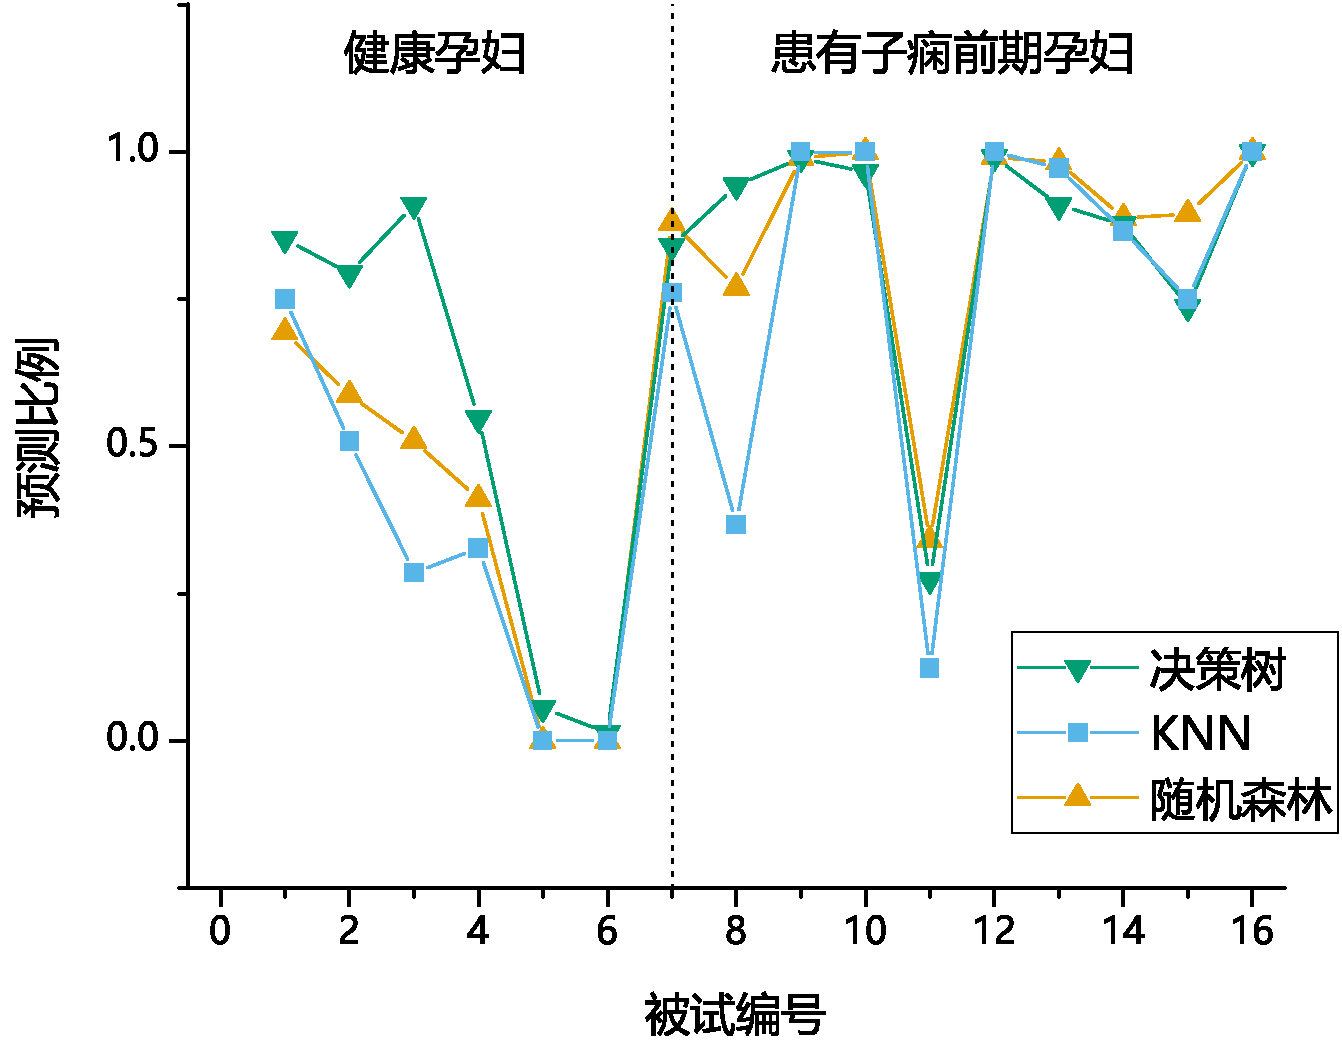
\includegraphics[width=7.5cm]{results/detail_31}
      }
      \quad
      \subfigure[\label{fig:detail_32}对脉搏波进行重采样处理得到的预测比例散点图]{
      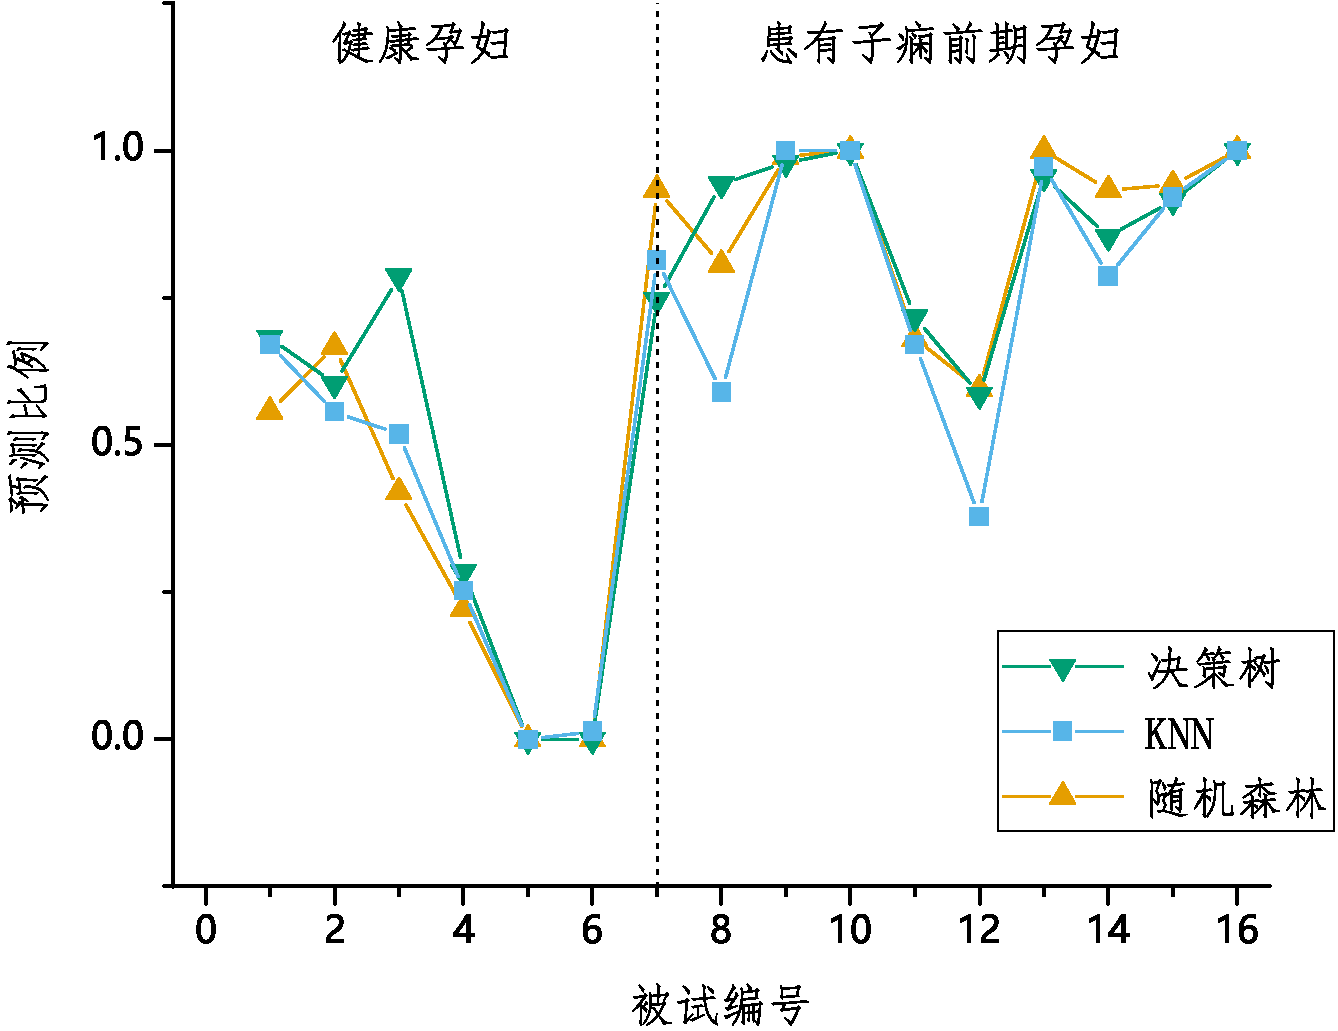
\includegraphics[width=7.5cm]{results/detail_32}
      }
      \caption{\label{fig:model_detail2}基于三种算法得到的子痫前期预测比例散点图2}
\end{figure}

\begin{figure}[htbp]
      \centering
      \subfigure[\label{fig:roc_31}按脉搏波进行补零处理得到的预测比例得到的ROC曲线]{
      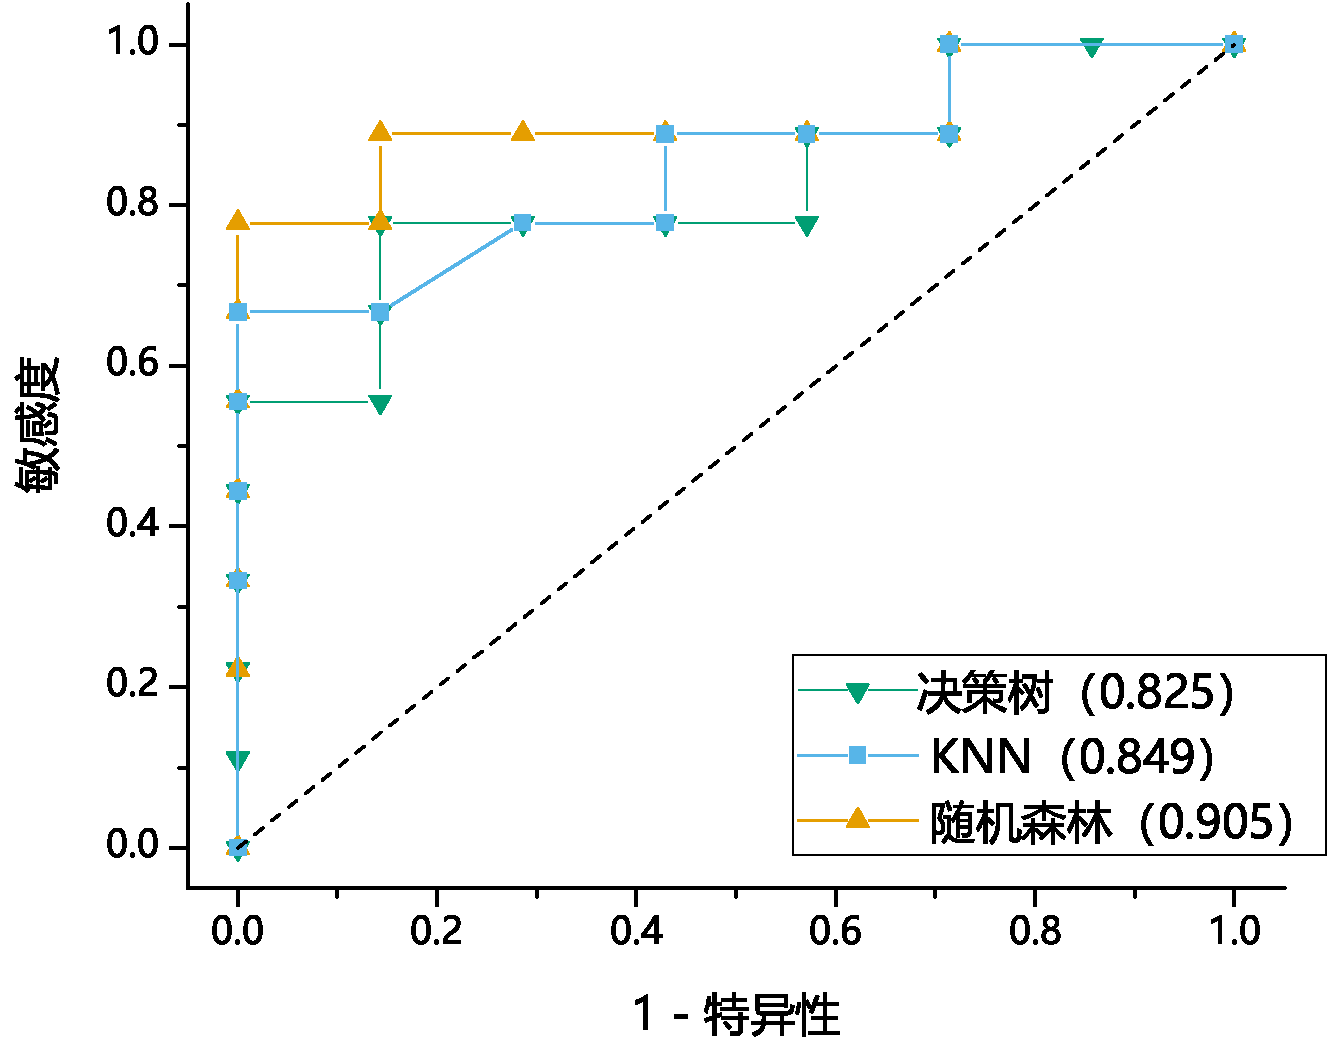
\includegraphics[width=7.5cm]{results/roc_31}
      }
      \quad
      \subfigure[\label{fig:roc_32}按脉搏波进行重采样处理得到的预测比例得到的ROC曲线]{
      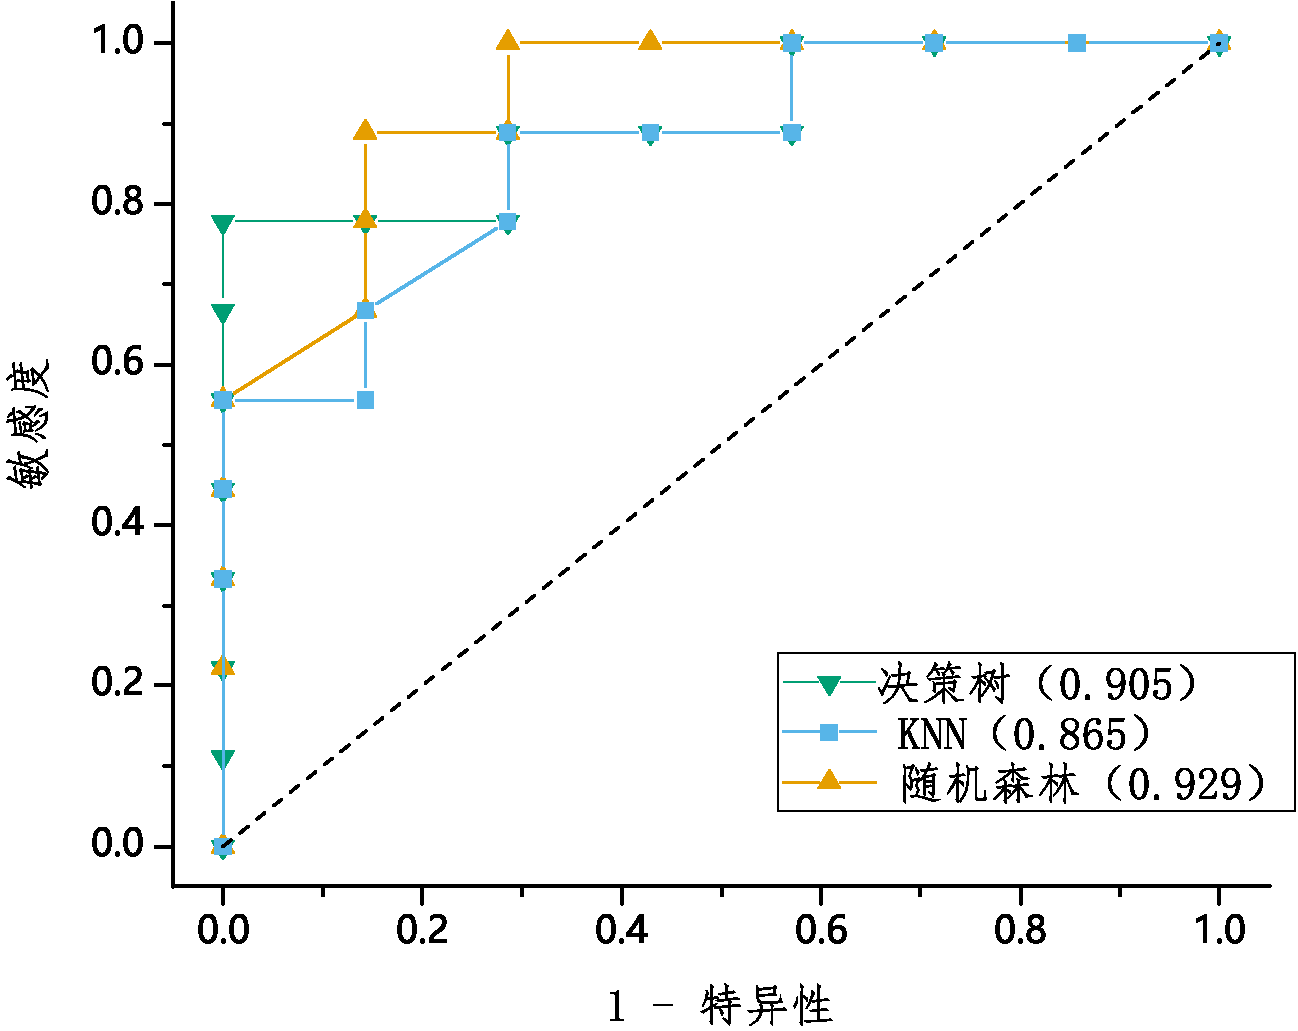
\includegraphics[width=7.5cm]{results/roc_32}
      }
      \caption{\label{fig:model_roc2}由子痫前期预测比例得到的 ROC 曲线2}
\end{figure}

% \vspace{-0.5cm} 
\begin{center}
      \zihao{-5}
      % \setlength{\belowcaptionskip}{-0.5cm} 
      \begin{longtable}{m{2.8cm}<{\centering}m{2.8cm}<{\centering}m{2cm}<{\centering}m{1.5cm}<{\centering}m{1.8cm}<{\centering}m{1.8cm}<{\centering}}
            \caption{三种模型在最佳分割阈值下的混淆矩阵}\\
            \label{tab:cm_on_best2}\\
            \topline
            \colorhead \textbf{机器学习算法}&\textbf{PPG对齐策略}&\textbf{最佳阈值}&\textbf{混淆矩阵}&\textbf{准确率}&\textbf{AUC}\\
            \midline
            \endfirsthead
            \caption[]{(续)}\\ 
            \topline
            \colorhead \textbf{机器学习算法}&\textbf{PPG对齐策略}&\textbf{最佳阈值}&\textbf{混淆矩阵}&\textbf{准确率}&\textbf{AUC}\\
            \midline
            \endhead 
            \midline
            \endfoot
            \bottomline
            \endlastfoot
            \colorrowa DT                              &     CS    & 0.864     &     $\left[ \begin{array}{cc} 7 & 2 \\ 1 & 6 \end{array} \right]$  & 81.3\% & 0.825 \\
            \colorrowa DT       &     RS      & 0.573     &     $\left[ \begin{array}{cc} 7 & 2 \\ 0 & 7 \end{array} \right]$  & 87.5\% & 0.905  \\
            \colorrowc KNN                              &     CS   & 0.813     &     $\left[ \begin{array}{cc} 6 & 3 \\ 0 & 7 \end{array} \right]$  & 81.3\% & 0.849  \\
            \colorrowc KNN        &     RS     & 0.820     &     $\left[ \begin{array}{cc} 8 & 1 \\ 2 & 5 \end{array} \right]$  & 81.3\% & 0.865 \\
            \colorrowa RF                              &     CS    & 0.884     &     $\left[ \begin{array}{cc} 7 & 2 \\ 1 & 6 \end{array} \right]$  & 81.3\% & 0.905  \\
            \colorrowa RF       &     RS      & 0.673    &     $\left[ \begin{array}{cc} 8 & 1 \\ 1 & 6 \end{array} \right]$  & 87.5\% & 0.929  \\
      \end{longtable}
\end{center}
\vspace{-0.8cm} 

从上述研究结果中可以得到以下结论:

1、在SR策略下基于PPGSTDS,按CS与RS等两种PPG对齐处理策略,借助DT、KNN与RF算法均可以训练得到性能较好的PE识别模型。

2、从识别准确率方面来看,三种算法训练得到的模型均可达到81.3\%以上,其中,DT与RF算法生成的模型性能接近,KNN算法得到的模型准确率最低。从AUC数值方面来看,RF算法有着最佳的分类效果,AUC数值最

\clearpage

\noindent
大(0.905与0.929)。

3、对比CS与RS等两种PPG对齐处理策略,两种策略下,三种算法在测试集上的混淆矩阵高度相似,识别准确率也基本保持一致。这也说明了两种处理策略本身的合理性。

4、从最佳分割阈值来看,使用CS对PPG波形对齐处理后,三种算法对应的分割阈值较大,有泛化能力不足的潜在风险;而使用RS对PPG波形对齐处理后,DT与RF算法得到的分割阈值则明显下降(0.573与0.673)。

\section{分析与讨论}
本小节在回顾前两节中及第四章的研究内容的基础上,从以下几个方面对上述处理分析得到的结果进行了分析与讨论。

一、两种猜想与两种验证猜想的方式

本文的研究目标是探寻通过PPG识别判断PE病发的可能,而该目标本质上可以划分为ML领域内的二分类任务。而本文对PPG与PE之间的可能潜在的关系,提出了以下两种猜想。

1、单个PPG波形可以反映PE的病发状态

这种猜想认为PPG的波形是孕妇PE病发状态的稳定“表达”,单个PPG波形包含了可以识别区分PE的全部信息。换言之,该猜想认为由PE导致的病生理变化可以在单个波形上得到全部体现,
单个PPG波形能够作为分析识别PE的最小分析对象。

2、被试的全部PPG波形才可以反映PE病发状态

这种猜想认为PPG的单个波形是孕妇PE病发状态的不稳定“表达”,但孕妇的一段时间内采集得到的所有PPG波形包含了可以识别区分PE的全部信息。换言之,该猜想认为由PE导致的病生理变化可以在孕妇
的多数PPG波形的形态特征上得到全部体现,需要被试的全部PPG波形进行一个类似“群体决策”的过程。

针对上述两个猜想,本研究从以下两个方向展开了具体研究工作:

1、基于波形的研究

基于波形的研究(pulse-based research,PR)将单个PPG波形作为分析识别PE的最小分析对象,并进行ML算法模型的研究。此研究方向下,同一被试的PPG数据可能对应ML模型训练与验证阶段的多个数据样本,这种方式相对地增加了
数据集的样本容量。

2、基于被试的研究

基于被试的研究(subject-based research,SR)将单个被试的所有PPG波形作为一个整体进行分析处理,并进行ML算法模型的研究。此研究方向下,同一被试的PPG波形只会出现在训练集或测试集之中,
测试集中的数据样本对于训练得到的模型是完全陌生的未见示例,因此更考验ML模型的泛化能力。

二、机器学习模型的影响

在经过多种ML算法的初筛后,前文中着重考察了通过DT、KNN与RF算法构建PE识别模型的效果。
对本文涉及的所有研究工作中涉及的基于上述三种算法模型训练得到的PE识别模型的在测试集上的准确率进行整理,结果如\autoref{tab:accuracy}所示。

\begin{center}
      \zihao{-5}
      % \setlength{\belowcaptionskip}{-0.5cm} 
      \begin{longtable}{m{1.5cm}<{\centering}m{1.5cm}<{\centering}m{2cm}<{\centering}m{1.5cm}<{\centering}m{1.5cm}<{\centering}m{1.5cm}<{\centering}m{2cm}<{\centering}}
            \caption{不同分析场景下通过三种算法模型在测试集上准确率对比}\\
            \label{tab:accuracy}\\
            \topline
            \colorhead \textbf{数据集}&\textbf{抽样方式}&\textbf{PPG对齐策略}&\textbf{随机森林}&\textbf{K近邻}&\textbf{决策树}&\textbf{备注}\\
            \midline
            \endfirsthead
            \caption[]{(续)}\\ 
            \topline
            \colorhead \textbf{数据集}&\textbf{抽样方式}&\textbf{PPG对齐策略}&\textbf{随机森林}&\textbf{K近邻}&\textbf{决策树}&\textbf{备注}\\
            \midline
            \endhead 
            \midline
            \endfoot
            \bottomline
            \endlastfoot
            \colorrowa PPGMTFS & PR & / &  97.0\% & 93.3\% &  88.9\%& / \\
            \colorrowa PPGMTFS & SR & / &  79.1\% & 78.3\% & 66.3\% & 按波形统计 \\
            \colorrowa PPGMTFS & SR & / &  93.8\% & 81.3\% & 81.3\% & 按被试统计 \\
            \colorrowc PPGSTFS & PR & CS &  93.6\% & 91.4\% & 86.2\% & / \\
            \colorrowc PPGSTFS & PR & RS &  92.5\% & 91.6\% & 83.9\% & /\\
            \colorrowc PPGSTFS & SR & CS &  74.3\% & 78.3\% & 67.5\% & 按波形统计\\
            \colorrowc PPGSTFS & SR & RS &  77.0\% & 74.7\% & 71.6\%& 按被试统计\\
            \colorrowc PPGSTFS & SR & CS &  81.3\% & 81.3\% & 81.3\%& 按波形统计\\
            \colorrowc PPGSTFS & SR & RS &  87.5\% & 81.3\% & 87.5\%& 按被试统计\\
      \end{longtable}
\end{center}
\vspace{-0.8cm} 

从\autoref{tab:accuracy}可以发现,在本研究涉及的多种分析场景下,RF算法充分体现了集成学习的优势,构建的模型性能均高于DT与KNN算法。
而对于DT与KNN算法而言,在大多数分析场景下,KNN算法的性能表现优于DT算法。

三、特征集的影响

进一步考察\autoref{tab:accuracy}中使用的数据集对PE识别模型在测试集上准确率,可以发现本文提出的PPGMTFS与PPGSTFS在PE的识别能力上具有一致性,这也说明PPGMTFS的设计合理性。
在相同的研究场景中,使用相同算法在两类特征集构建的模型在测试集上的准确率数值极为接近,且均是在PPGMTFS上的构建模型性能优于在PPGMSFS上构建的模型。
这也表明,PPGMTFS表征PE的能力要强于PPGSTFS,换言之,PPGMTFS中包含了与PE相关性更强的描述特征。

四、特征贡献与分布

使用RF算法在PPGMTFS与PPGSTFS上构建模型时,可以评估参与模型构建的特征的贡献度。
对比\autoref{tab:rf_dr_1}与\autoref{fig:rf_imp2},可以发现:

1、PPGMTFS与PPGSTFS中特征贡献度的最大数值有一定差异,前者可以到达整体平均值的13.6倍以上,而后者仅为均值的6倍左右。这也说明在PPGMTFS中,与PE相关的特征更为明显。

2、对比两种特征集上得到各特征的贡献度分布可以发现,两类时域特征集中具有PE表征能力的特征出现的位置高度相似。贡献度高的特征多出现在下降支中,且集中在下降支的前端与尾端。这点在
\autoref{fig:rf_imp2}体现得更为明显,在特征贡献度分布中,脉搏波峰值之后及尾端位置出现了两个分布高峰。这种现象也与PPG
下降支是血液回流过程的反应、下降支包含了更多的血液循环中细节信息的、PE
会影响孕妇血液循环等事实相符合。同时也表明这些位置的PPG形态可能是识别PE的关键。

\section{小结}
本章在PPGMTFS与PPPGSTFS等数据集的基础上,按照基于波形与基于被试等两个研究方向,对单个PPG波形可以反映PE的病发状态与被试的全部PPG波形才可以反映PE病发状态等两个猜想进行了验证。
利用ML的多种监督学习算法,完成了包括多算法模型筛选、模型超参数优化、特征贡献度分析与降维处理等研究分析工作,构建了多种PE识别模型与并对结果进行了分析。
这些结果表明,同时,本文构建的PPGMTFS与PPPGSTFS等数据集设计合理,具有能表征PE的关键特征。与此同时,基于这些PPG数据集,通过ML算法构建PE识别模型具有一定的可行性。
